
\chapter{Fractions}




\fellow{Formatting: can we put things marked ``Problem'' in a box (maybe with some color?) to set it apart?  Same with the Think/Pair/Share (different color?) and Solutions.}

Fractions are one of the hardest topics to teach (and learn!) in elementary school.  What is the reason for this?  We'll try to provide some insight in this chapter, along with some better ways for understanding, teaching, and learning about fractions.  But for now, talk with a partner about what makes this topic so hard.


\begin{thinkpair*}
You may have struggled learning about fractions in elementary school.  Maybe you still find them confusing.  Even if you were one of the lucky ones who didn't struggle when learning about fractions, you probably had friends who did struggle.

With a partner, talk about why this is.  What is so difficult about understanding fractions?  Why is the topic harder than other ones we tackle in elementary schools?
\end{thinkpair*}

Remember that teachers should have lots of mental models --- lots of ways to explain the same concept.  In this chapter, we'll look at some different ways to understand the idea of fractions as well as basic operations on them. 



\section{What is a Fraction?}
One of the things that makes fractions such a difficult concept to teach and to learn is that you have to think about them in lots of different ways, depending on the problem at hand.
For now, we're going to think of a fraction as the answer to a division problem.  

\fellow{Throughout: anything you can do to make the pictures better would be awesome.}

\begin{example}[Pies per boy]
Suppose 6 pies are to be shared equally among 3 boys. This yields 2
pies per boy. We write:
\[
\frac 6 3 = 2.
\]


\begin{center}
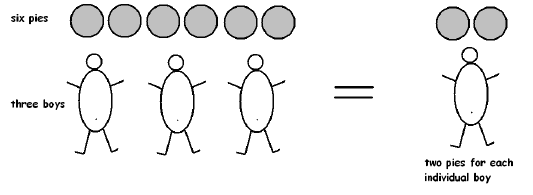
\includegraphics[height = 4cm]{PPB1}
\end{center}

The fraction $\frac 6 3$ is equivalent to the answer to the division problem $6 \div 3 = 2$.  It represents the number of pies one whole boy receives. 
\end{example}

In the same way \dots

\begin{itemize}
\item[]
sharing 10 pies among 2 boys yields $ \frac{10}2 = 5 $ pies per boy,\\
\item[]
sharing 8 pies among 2 boys yields $ \frac{8}2 = 4 $ pies per boy,\\
\item[]
sharing 5 pies among 5 boys yields $ \frac{5}5 = 1 $ pies per boy, and\\


\item[]
the answer to sharing 1 pies among 2 boys is $ \frac{1}2 $, which we call ``one-half.''


\end{itemize}


This final example is actually saying something! It also represents how fractions are
usually taught to students:

\begin{quotation}
\emph{
If one pie is shared (equally) between two boys, then each boy receives a portion of
a pie which we choose to call ``half.''}
\end{quotation}

\begin{center}
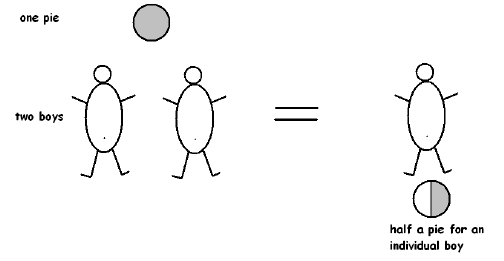
\includegraphics[height = 5cm]{PPB2}
\end{center}



Thus students are taught to associate the number ``$\frac 1 2$'' to the picture

\includegraphics[height = 15pt]{halfpie}.

In the same way, the picture 
\includegraphics[height = 15pt]{thirdpie} is said to represent ``one third,'' that is,
$ \frac 1 3$.
(And this is indeed the amount of pie an individual boy would receive if one pie is
shared among three.)


The picture

\includegraphics[height = 15pt]{fifthpie}
 is called ``one fifth'' and is indeed
$\frac 1 5$, the amount of pie an
individual boy receives when one pie is shared among five.
 
And the picture
 
\includegraphics[height = 15pt]{3fifthpie}
 is called ``three fifths'' to represent
$\frac 3 5$,
the amount of pie
an individual receives if three pies are shared among five boys.
 
 \begin{thinkpair*}
 Carefully explain \emph{why} this is true: If five boys share three pies equally, each boy receives an amount that looks like this:  
\includegraphics[height = 15pt]{3fifthpie}.  Your explanation will probably require both words and pictures.

 \end{thinkpair*}
 
 
\subsection*{On Your Own}
 Work on the following exercises on your own or with a partner.
 
 \begin{enumerate}
 \item
 Draw a picture associated with the fraction $ \frac 1 6$.\\
 
 \item
Draw a picture associated with the fraction $ \frac 3 7$.
Is your picture
really the amount of pie an individual boy would receive if three pies are shared
among seven boys? Be very clear on this!\\

\item
Let's work backwards! Here is the answer to a division problem:
\begin{center}
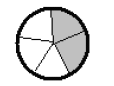
\includegraphics[height = 2cm]{2fifthspie}
\end{center}
This represents the amount of pie an individual boy receives if some number of pies
is shared among some number of boys.  How many pies?  How many boys?  How can you justify your answers?\\

\item
Here is another answer to a division problem:
\begin{center}
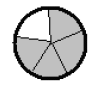
\includegraphics[height = 2cm]{4fifthspie}
\end{center}
How many pies?  How many boys?  How can you justify your answers?\\


\item
Here is another answer to a division problem:
\begin{center}
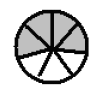
\includegraphics[height = 2cm]{4seventhspie}
\end{center}
How many pies?  How many boys?  How can you justify your answers?\\

\item
Leigh says that ``$\frac 3 5$ is three times as big as $\frac 1 5$.''
Is this right? Is
three pies shared among five boys three times as much as one pie shared among
five boys? Explain your answer.\\

\item
Draw a picture for the answer to the division problem $\frac 4 8$.
Describe
what you notice about the answer.\\

\item
Draw a picture for the answer to the division problem $\frac 2 {10}$.
Describe
what you notice about the answer.\\

\item
What does the division problem $\frac 1 1$
represent? How much pie does an
individual boy receive?\\


\item
What does the division problem $\frac 5 1$
represent? How much pie does
an individual boy receive?\\

\item
What does the division problem $\frac 5 5$
represent? How much pie does
an individual boy receive?\\



\item
Here is the answer to another division problem. This is the amount
of pie an individual boy receives:
\begin{center}

\includegraphics[height = 2cm]{3halfpie}
\end{center}
How many pies were in the division problem?  How many boys were in the division problem?  Justify your answers.\\


\item
Here is the answer to another division problem. This is the amount
of pie an individual boy receives:
\begin{center}
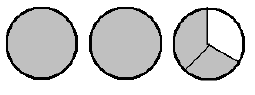
\includegraphics[height = 2cm]{8thirdpie}
\end{center}
How many pies were in the division problem?  How many boys were in the division problem?  Justify your answers.\\



\item
Many teachers have young students divide differently shaped pies
into fractions. For example, a hexagonal pie is good for illustrating the fractions
\[
\frac 1 6, \quad
\frac 2 6, \quad
\frac 3 6, \quad
\frac 4 6, \quad
\frac 5 6, \text{ and }\quad
\frac 6 6.
\]

\begin{center}
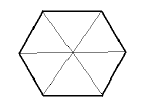
\includegraphics[height = 2cm]{hexpie}
\end{center}


\begin{enumerate}
\item
Why is this shape used?  What does $\frac 1 6$ of a pie look like?

\item
What does $\frac 6 6 $ of a pie look like?

\item
What shape pie would be good for illustrating the fractions $\frac 1 8 $ up to $\frac 8 8$?
\end{enumerate}

 \end{enumerate}
 
 
 
 
 \begin{problem}
 Some rectangular pies are distributed to some number of boys. This picture
represents the amount of pie an individual boy receives.
 \begin{center}
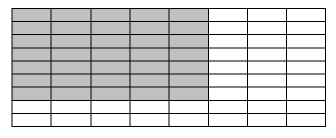
\includegraphics[height = 2.5cm]{rectpie}
\end{center}
 How many pies?  How many boys?  Carefully justify your answers!
 
 \end{problem}
 
 
 
 
\subsection{Pies Per Boy Model}
In our model, a fraction
$\frac a b$ represents the amount of pie an individual boy
receives when $a$ pies are shared equally by  $b$ boys.
  \begin{center}
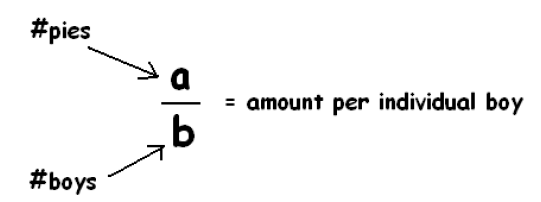
\includegraphics[height = 3cm]{PPBmodel}
\end{center}

\begin{thinkpair*}\ 

\begin{enumerate}
\item
What is $\frac 2 2$?  What is $\frac 7 7 $?  What is $\frac{100}{100}$?  How can you use the ``Pies Per Boy Model'' to make sense of $\frac a a$ for any positive whole number $a$?\\

\item
What is $\frac 2 1$?  What is $\frac 7 1 $?  What is $\frac{1876}{1}$?  How can you use the ``Pies Per Boy Model'' to make sense of $\frac b 1$ for any positive whole number $b$?\\

\item
Write the answer to this division problem: ``I have no pies to share among thirteen boys.''  How can you generalize this division problem to make a general statement about fractions?

\end{enumerate}

\end{thinkpair*}
 
 \begin{define}
 For a fraction $\frac a b$,
the top number $a$ (which, for us, is the number of pies) is called
the {\bf numerator} of the fraction, and the bottom number $b$ (the number of pies), is called the
{\bf denominator} of the fraction. 
 \end{define}
 
 Most people insist that the numerator and denominator  each be whole
numbers, but they really don't have to be.
 
 
  \begin{thinkpair*}
 To understand why the numerator and denominator need not be whole numbers, we must first  be a little gruesome.  Instead of dividing pies, let's divide boys!  Here is one boy:
  \begin{center}

\includegraphics[height = 2.5cm]{oneboy}
\end{center}

 \begin{itemize}
 \item
 What would half a boy look like?
 
 \item
 What would one-third of a boy look like?
 
 \item
 What would three-fifths of a boy look like?
 \end{itemize}
 
 \end{thinkpair*}


So, what would 
\[
\frac 1 {\left( \frac 1 2\right) }
\]
 represent?
 This means assigning one pie to each ``group'' of half a boy. So how much would a
whole boy receive?  Well, we would have a picture like this:
   \begin{center}
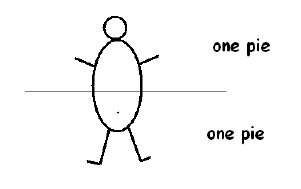
\includegraphics[height = 3cm]{halfboy}
\end{center}
The whole boy gets two pies,
so we have
\[
\frac 1 {\left( \frac 1 2\right) }
= 2.
\]



\begin{thinkpair*}
Draw pictures for these problems if it helps!

\begin{enumerate}
\item
What does 
\[
\frac 1 {\left( \frac 1 3\right) }
\]
represent?  Justify your answer using the ``Pies Per Boy Model.''\\

\item
What is  
\[
\frac 1 {\left( \frac 1 6\right) }?
\]
Justify your answer.\\


\item
Explain why  the fraction
\[
\frac 5 {\left( \frac 1 2\right) }
\]
represents the number 10.  (How much pie is given to half a boy?  To a whole boy?)\\


\item
What is  
\[
\frac 4 {\left( \frac 1 3\right) }?
\]
Justify your answer.\\

\item{\bf Challenge:}
Two-and-a-half pies are to be shared equally among four-and-a-half boys.  How much pie does an individual (whole) boy receive?  Justify your answer.
  \begin{center}
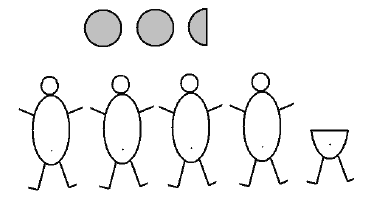
\includegraphics[height = 3.5cm]{5ninthspie}
\end{center}




\end{enumerate}

\end{thinkpair*}




\subsection{Jargon}
A fraction with a numerator smaller than its denominator is called (in school math jargon) a \emph{proper
fraction}. For example, $\frac {45}{58}$ is ``proper.''

A fraction with numerator larger than its denominator is called (in school math jargon) an \emph{improper
fraction}. 
For example, $\frac 7 3$ 
is  ``improper.'' (In the 1800s, these fractions were
called \emph{vulgar fractions}. Despite nineteenth-century views they are useful
nonetheless!)

For some reason, improper fractions are considered,
well, improper by some teachers.  So students are often asked to write improper fractions
as a combination of a whole number and a proper fraction.

Consider, for example,
$\frac 7 3$.
If seven pies are shared among three boys, then each boy
will certainly receive 2 whole pies, leaving one pie over to share among the three
boys. Thus, 
$\frac 7 3 $
equals 2 plus $\frac 1 3$.

People write:
\[
\frac 7 3 = 2\frac 1 3
\]
and call the result $2 \frac 1 3$
a \emph{mixed number}. (One can also write
\[
2 + \frac 1 3,
\]
which is what $2\frac 1 3$
really means.  But most people choose to suppress the plus sign.)

As another example, consider $\frac{23}4$.
If 4 boys share 23 pies, we can give them each five whole pies.  That uses 20 pies, and there
are then  3 pies left over.  Those three pies are still be shared equally by the 4 boys. We have:
\[
\frac{23}4 = 5\frac 3 4.
\]


Mathematically, there is nothing wrong with an improper fraction.  (In fact, many
mathematicians prefer improper fractions over mixed numbers.  They are often easier to use in computations.)
Consider, for instance, the mixed number $2\frac 1 5$.  This is really $2 + \frac 1 5$.

For fun, let's write the number 2 as a fraction with denominator five:
\[
2 = \frac{10} 5.
\]

So:
\[
2\frac 1 5 
\quad=\quad 2 + \frac 1 5 
\quad=\quad
 \frac{10} 5 + \frac{1} 5 
 \quad=\quad
  \frac{11}5.
\]

We've written the mixed number $2\frac 1 5$
as the improper fraction $\frac{11}5$.


\begin{thinkpair*}\ 
\begin{itemize}
\item
Write each of the following as a mixed number. Explain how you got your answer.
\[
\frac{17}3,
\qquad\qquad
\frac 8 5,
\qquad\qquad
\frac{100}{13},
\qquad\qquad
\frac{200}{199}.
\]

\item
Convert each of these mixed numbers  into ``improper'' fractions.  Explain how you got your answer.
\[
3\frac 1 4 ,
\qquad\qquad
5 \frac 1 6,
\qquad\qquad
1 \frac 3{11},
\qquad\qquad
200 \frac 1{200}.
\]
\end{itemize}

\end{thinkpair*}


Students are often asked to memorize the names ``proper fraction,''
``improper fraction'' and ``mixed number'' so that they can follow directions on tests
and problem sets.

But, to a mathematician, these names are not at all important!
There is no ``correct'' way to express an answer (assuming, that the answer is
mathematically the right number).  We often wish to express our answer in a simpler form, but sometimes the context will tell you what form is ``simple'' and what form is more complicated.

As you work on problems in this chapter, decide for yourself  which type of fraction would
be best to work with as you do your task.



\section{The Key Fraction Rule}
We know that $\frac a b$
is the answer to a division problem:
\begin{quotation}
$\displaystyle\frac a b $
represents the amount of pie an individual boy receives when $a$ pies are
distributed among $b$ boys.
\end{quotation}
What happens if we double the number of pies and double the number of boys?
Nothing! The amount of pie per boy is still the same:
\[
\frac{2a}{2b} = \frac a b.
\]
For example, as the picture shows,
$\frac 6 3$ and
$\frac{12} 6$
both give two pies for each boy.
 
   \begin{center}
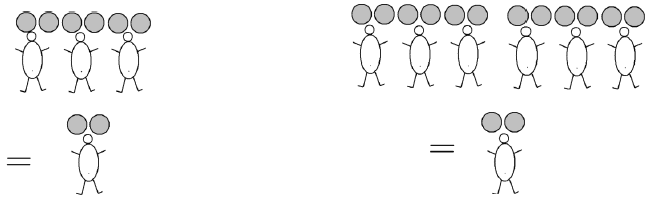
\includegraphics[height = 3.5cm]{PPBreduce}
\end{center}

And tripling the number of pies and tripling the number of boys also does not
change the final amount of pie per boy, nor does quadrupling each number, or onetrillion-
billion-tupling the numbers!
\[
\frac 6 3
= 
\frac{12} 6 = 
\frac {18}9 =
\cdots =
\text{ two pies per boy}.
\]

   \begin{center}
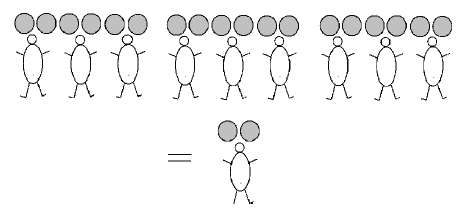
\includegraphics[height = 4cm]{PPBreduce2}
\end{center}


This leads us to want to believe:

\fellow{put this in a box and centered?}

{\bf Key Fraction Rule:} $\displaystyle \frac{xa}{xb} = \frac{a}{b}$ (at least for positive whole numbers $x$).


\begin{example}[Fractions equivalent to $\frac 35$]
 For example,
 $\frac 3 5$
(sharing three pies among five boys)
yields the same result as
 \[
 \frac{3 \cdot 2}{5 \cdot 2} = \frac{6}{10}
\text{ (sharing six pies among ten boys),}
 \]
and as
 \[
 \frac{3 \cdot 100}{5 \cdot 100} = \frac{300}{500}
\text{ (sharing 300 pies among 500 boys).}
 \]
 \end{example}
 
 
 \begin{thinkpair*}
Write down lots of equivalent fractions for $\frac 1 2$,  for $\frac {10}3$, and for~$1$.  
 \end{thinkpair*}
 
  
\begin{example}[Going backwards]
 \[
 \frac{20}{32}
\text{ (sharing 20 pies among 32 boys)}
 \]
is the same problem as:
 \[
\frac{5 \cdot 4 }{8\cdot 4} = \frac 5 8
\text{ (sharing five pies among eight boys).}
 \]
 \end{example}
 
 
Most people say we have \emph{cancelled} or taken a common factor of 4 from
the numerator and the denominator.
 
Mathematicians call this process \emph{reducing} the fraction to lowest terms. (We've
made the numerator and denominator each smaller, in fact as small as we can make them!) 
 
 Teachers tend to say that we
are \emph{simplifying} the fraction. (You have to admit that $\frac 5 8$
does look simpler than
$\frac{20}{32}$.)
 
 
 \begin{example}[How low can you go?]
 As another example,
 $\frac{280}
{350}$
can certainly be simplified by noticing that there is a
common factor of $10$ in both the numerator and the denominator:
 \[
 \frac{280}{350} = \frac{28\cdot 10}{35\cdot 10} = \frac{28}{35}.
 \]
We can go further as 28 and 35 are both multiples of 7:
 \[
 \frac{28}{35} = \frac{4 \cdot 7}{4 \cdot 7} = \frac 4 5.
 \]
Thus, sharing 280 pies among 350 boys gives the same result as sharing just 4 pies
among 5 boys!
\[
 \frac{280}{350} = \frac 4 5.
 \]
Since 4 and 5 share no common factors, this is as far as we can go with this example
(while staying with whole numbers!).
 \end{example}
 
 \begin{thinkpair*}
 Jenny says that $\frac 4 5$
does ``reduce'' further is you are willing to move
away from whole numbers. She writes:
 \[
 \frac{4}{5} = 
 \frac{2\cdot 2}{\left(2\frac 1 2\right) \cdot 2}=
 \frac{2}{\left(2\frac 1 2\right)}.
 \]
Is she right? Does sharing 4 pies among 5 boys yield the same result as sharing 2
pies among $2\frac 1 2$ boys?
What do you think?
 
 \end{thinkpair*}
 


\subsection*{On Your Own}
Mix and Match: On the top are some fractions that have not
been simplified. On the bottom are the simplified answers, but in random order.
Which simplified answer goes with which fraction? (Notice that there are fewer
answers than questions!)

\[
{\bf 1.} \frac{10}{20} 
\qquad\qquad
{\bf 2.} \frac{50}{75} 
\qquad\qquad
{\bf 3.} \frac{24000}{36000} 
\qquad\qquad
{\bf 4.} \frac{24}{14} 
\qquad\qquad
{\bf 5.} \frac{18}{32} 
\qquad\qquad
{\bf 6.} \frac{1}{40} 
\]

\[
{\bf a.} \frac{2}{3} 
\qquad\qquad
{\bf b.} \frac{9}{16} 
\qquad\qquad
{\bf c.} \frac{12}{7} 
\qquad\qquad
{\bf d.} \frac{1}{40} 
\qquad\qquad
{\bf e.} \frac{1}{2} 
\]


\begin{thinkpair*}
Use the ``Pies Per Boy Model'' to explain \emph{why} the key fraction rule holds.  That is, explain why each individual boy gets the same amount of pie in these two situations:
\begin{itemize}
\item
 if you have $a$ pies and $b$ boys, or
 \item
  if you have $xa$ pies and $xb$ boys.
  \end{itemize}
\end{thinkpair*}





\section{Adding and Subtracting Fractions}

\subsection{Fractions with the Same Denominator}

Here are two very similar fractions:
$\frac 2 7$ and $\frac 3 7$.
What might it mean to add them?
It might be tempting to say:
\begin{align*}
\frac 2 7 &
\text{ represents 2 pies being shared among 7 boys}\\
\frac 3 7 &
\text{ represents 3 pies being shared among 7 boys}\\
\end{align*}
so
$\frac 2 7 + \frac 3 7$ 
probably represents sharing 5 pies among 14 boys, giving the answer
$\frac 5{14}$.
That is, it is very tempting to say that ``adding fractions'' means  ``adding pies and 
adding boys.''

The trouble is that a fraction is not a pie, and a fraction is not a boy. So adding
pies and adding boys is {\bf not} actually adding fractions. 
A fraction is something
different. It is related to pies and boys, but something more subtle. A fraction is
an amount of {\bf pie per boy}.

One can't add pies, one can't add boys. One must add instead the amounts individual
boys receive.

\begin{example}[$\frac 27 + \frac 37$]
Let's take it slowly.
Consider the fraction $\frac 2 7$.
Here is a picture of the amount an individual boy receives when two pies are given to seven boys:
   \begin{center}
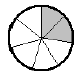
\includegraphics[height = 2cm]{2seventhspie}
\end{center}



Consider the fraction $\frac 3 7$.
Here is a picture of the amount an individual boy receives
when three pies are given to seven boys:
   \begin{center}
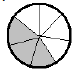
\includegraphics[height = 2cm]{3seventhspie}
\end{center}


The sum
$\frac 2 7 + \frac 3 7 $
corresponds to the sum:

   \begin{center}
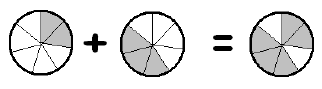
\includegraphics[height = 2.5cm]{addseventhspie}
\end{center}



The answer, from the picture, is $\frac 5 7$.
\end{example}

\begin{thinkpair*}
Remember that $\frac 5 7$ means ``the amount of pie that one boy gets when five pies are shared by seven boys.''  Carefully explain \emph{why} that is the same as the picture given by the sum above:
    \begin{center}

\includegraphics[height = 2cm]{sumseventhspie}
\end{center}
Your explanation should use both words and pictures!


\end{thinkpair*}




Most people read this as ``Two sevenths plus three sevenths gives five sevenths''
and think that the problem is just as easy as saying ``two apples plus three apples
gives five apples.'' And, in the end, they are right!
   \begin{center}
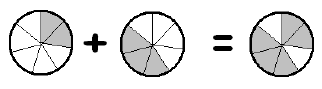
\includegraphics[height = 2.5cm]{addseventhspie}
\[
\frac 2 7 + \frac 3 7 = \frac 5 7.
\]
\end{center}

This is how the addition of fractions is first taught to students: Adding fractions
with the same denominator seems just as easy as adding apples:


\begin{align*}
4 \text{ tenths} + 3 \text{ tenths} + 8 \text{ tenths} & = 15 \text{ tenths}\\
\frac 4 {10} + \frac 3 {10} + \frac 8 {10} &= \frac{15}{10}.
\end{align*}

(And, if you like,
$\frac{15}{10} = \frac{5\cdot 3}{5\cdot 2} = \frac 3 2$.)


\begin{align*}
82 \text{ sixty-fifths} + 91 \text{ sixty-fifths} & = 173 \text{ sixty-fifths}\\
\frac {82} {65} + \frac {91} {65}  &= \frac{173}{65}.
\end{align*}

We are really adding {\bf amounts per boy} not amounts, but the answers match the same way.

We can use the ``Pies Per Boy Model'' to explain \emph{why}  adding fractions with like denominators works in this way.  

Think about the addition problem $\frac 2 7 + \frac 3 7$:
\begin{align*}
&\text{ amount of pie each boy gets when 7 boys share 2 pies} \\
+ 
&\text{\underline{ amount of pie each boy gets when 7 boys share 3 pies} }\\ 
&???
\end{align*}
Since in both cases we have 7 boys sharing the pies, we can imagine that it's the same 7 boys in both cases.  First they share 2 pies.  Then they share 3 more pies.  The total each boy gets by the time all the pie-sharing is done is the same as if the 7 boys had just shared 5 pies to begin with.  That is:
\begin{align*}
&\text{ amount of pie each boy gets when 7 boys share 2 pies} \\
+ 
&\text{\underline{ amount of pie each boy gets when 7 boys share 3 pies} }\\ 
&\text{ amount of pie each boy gets when 7 boys share 5 pies}\\ 
\end{align*}
\[
\frac 2 7 + \frac 3 7 = \frac 5 7.
\]

Now let's think about the general case.  Our claim is that
\[
\frac a d + \frac b d = \frac{a+b}d.
\]
Translating into our model, we have $d$ boys.  First, they share $a$ pies between them, and $\frac a d$ represents the amount each boy gets.  Then they share $b$ more pies, so the additional amount of pie each boy gets is $\frac b d$.  The total each boy gets is $\frac a d + \frac b d$.

But it doesn't really matter that the boys first share $a$ pies and then share $b$ pies.  The amount each boy gets is the same as if they had started with all of the pies --- all $a+b$ of them --- and shared them equally.  That amount of pie is represented by $\frac{a+b}d$.  



\begin{thinkpair*}\ 
\begin{enumerate}
\item
How can you \emph{subtract} fractions with
the same denominator? For example, what is
\[
\frac{400 }{903} -\frac{170}{903}?
\]

\item
Use the ``Pies Per Boy'' model to \emph{carefully explain why}
\[
\frac a d - \frac b d = \frac{a-b}{d},
\]
at least if $b \leq a$ and everything in sight is a positive whole number.

\item
Explain why the fact that the denominators are the same is \emph{essential} to this addition and subtraction method.  Where is that fact used in the explanations?
\end{enumerate}
\end{thinkpair*}


\subsection{Fractions with Different Denominators}

This approach to adding fractions suddenly becomes tricky if the denominators
involved are not the same common value. For example, what is
$\frac 2 5 + \frac 1 3$?

   \begin{center}
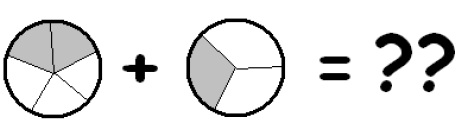
\includegraphics[height = 2cm]{addingfrac1}
\end{center}


Let's phrase this question in terms of pies and boys:

\begin{quotation}
\emph{Suppose Poindexter is part of a team of a five boys that receives two pies.
Then later he is part of a team of three boys that receives one pie. How much pie does
Poindexter receive in total?}
\end{quotation}

\begin{thinkpair*}
Talk about these questions with a partner before reading on. It is actually a very difficult problem!  What might a student say, if they don't already know about adding fractions?  Write down any of your thoughts.
\begin{enumerate}
\item
Do you see that this is the same problem as computing $ \frac 2 5 + \frac 1 3$?
\item
What might be the best approach to answering this problem?
\end{enumerate}

\end{thinkpair*}



One way to think about answering this addition question is to write
$\frac 2 5$
in a series of
alternative forms using our fraction rule (that is, multiply the numerator and
denominator each by 2, and then each by 3, and then each by 4, and so on) and to do
the same for
$\frac 1 3$:

\begin{align*}
\frac 2 5 \quad + &\quad  \frac 1 3\\
\\
\frac 4{10}\quad \phantom {+} & \quad \frac 2 6\\
\\
{\color{red} \frac 6{15}}\quad \phantom {+} & \quad \frac 3 9\\
\\
\frac 8{20}\quad \phantom {+} & \quad \frac 4 {12}\\
\\
\frac {10}{25}\quad \phantom {+} & \quad {\color{red} \frac 5 {15}}\\
\\
\vdots \qquad &\quad \vdots
\end{align*}
We see that the
problem $\frac 2 5 + \frac 1 3$ 
is actually the same as $\frac 6{15} + \frac5{15}$.  So we can find the answer using the same-denominator method:
\[
\frac 2 5 + \frac 1 3 
\quad = \quad
\frac 6{15} + \frac 5{15}
 \quad = \quad 
 \frac{11}{15}.
\]



\begin{example}[$\frac 38 + \frac 3{10}$]
Here's another example of adding fractions with unlike denominators: $\frac 38 + \frac 3{10}$.  In this case, Poindexter is first part of a group of 8 boys who share 3 pies.  Later he is part of a group of 10 boys who share 3 different pies.  How much total pie did Poindexter get?

\begin{align*}
\frac 38 \quad + &\quad  \frac 3{10}\\
\\
\frac 6{16}\quad \phantom {+} & \quad \frac 6 {20}\\
\\
 \frac 9{24}\quad \phantom {+} & \quad \frac 9 {30}\\
\\
\frac {12}{32}\quad \phantom {+} & \quad {\color{red} \frac  {12}{40}}\\
\\
{\color{red} \frac {15}{40}}\quad \phantom {+} & \quad \frac  {15}{50}
\\
\vdots \qquad &\quad \vdots
\end{align*}
\[
\frac 38  +   \frac 3{10} 
\quad = \quad
 \frac{15}{40} + \frac{12}{40} 
 \quad = \quad
  \frac{17}{40}.
\]


\end{example}

Of course, you don't need to list \emph{all} of the equivalent forms of each
fraction in order to find a common denominator. If you can see a common
denominator right away (or can think of a faster method that always works), go for it!

\begin{thinkpair*}
Cassie suggests the following method for the example above:

\begin{quotation}
\emph{When the denominators are the same, we just add the numerators.  So when the numerators are the same, shouldn't we just add the denominators?  Like this: $\frac 38 + \frac 3{10} = \frac 3{18}$.
}\end{quotation}

What do you think of Cassie's suggestion?  Does it make sense?  What would you say if you were Cassie's teacher?
\end{thinkpair*}



\subsection*{On Your Own}
Try these exercises on your own.  For each addition exercise, also write down a ``Pies Per Boy'' interpretation of the problem.  You might also want to draw a picture.

\begin{enumerate}
\item
What is $\frac 1 2 + \frac 1 3$?\\

\item
What is $\frac 2 5 + \frac {37}{10}$?\\

\item
What is $\frac 1 2 + \frac 3{10}$?\\

\item
What is $\frac 2 3 + \frac 5 7 $?\\

\item
What is $\frac 1 2 + \frac 1 4 + \frac 1 8$?\\

\item
What is $\frac 3{10} + \frac 4{25} + \frac 7{20} + \frac 35 + \frac{49}{50}$?\\
\end{enumerate}

Now try these subtraction exercises.
\begin{enumerate}
\addtocounter{enumi}{6}

\item
What is $\frac 7{10} - \frac 3{10}$?\\

\item
What is $\frac 7{10} - \frac {3}{20}$?\\

\item
What is $\frac 1 3 - \frac 1{5}$?\\

\item
What is $\frac 2 {35} - \frac 2 7 + \frac 2 5 $?\\

\item
What is $\frac 1 2 - \frac 1 4 - \frac 1 8 - \frac 1 {16}$?\\
\end{enumerate}


\begin{thinkpair*}
Which fraction is larger, $\frac 5 9 $ or $\frac 6{11}$?  Justify your answer.
(Oh, and what does this question have to do with the subject of this section: adding and subtracting fractions?)
\end{thinkpair*}





\section{What is a Fraction? Revisited}
So far, we've been thinking about a fraction as the answer to a division problem.  For example,  $\frac 2 3$ is the result of sharing two pies among three boys.

   \begin{center}
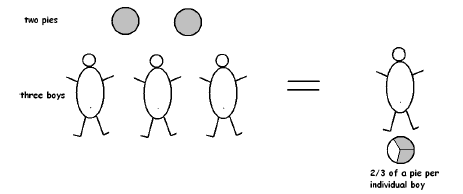
\includegraphics[height = 4.5cm]{2pies3boys}
\end{center}

Of course, pies don't have to be round.  We can have square pies, or triangular pies or squiggly pies or any shape you please.


   \begin{center}
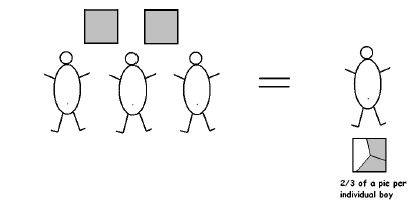
\includegraphics[height = 4.5cm]{2pies3boys2}
\end{center}


This ``Pies Per Boy Model'' has served us perfectly well in thinking about the meaning of fractions, equivalent fractions, and even adding and subtracting fractions. 

However, there's not any way to use this model to make sense of multiplying fractions!  What would this mean?

   \begin{center}
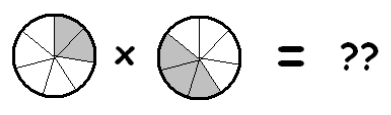
\includegraphics[height = 2cm]{PPBtimes}
\end{center}

So what are fractions, if we are  asked to multiply them?  We are forced to switch models and think about fractions in a new way.

 This switch of gear is fundamentally perturbing: Does a fraction have anything to do with pie or pies per boy or not? If the answer is that a fraction is more of an abstract concept that applies simultaneously to pies and boys and to something else that we can multiply, then what is that concept exactly? 

Think about our poor young students. We keep switching concepts and models, and speak of fractions in each case as though all is naturally linked and obvious. All is not obvious and all is absolutely confusing.
 This is just one of the reasons that fractions can be such a difficult concept to teach and to learn in elementary school!


\begin{thinkpair*}[What's wrong here?]
For each of the following visual representations of fractions, there is a corresponding \emph{incorrect} symbolic expression.   Discuss with your partner: why is the symbolic representation incorrect?  What might elementary students find confusing in these visual representations?

\begin{center}
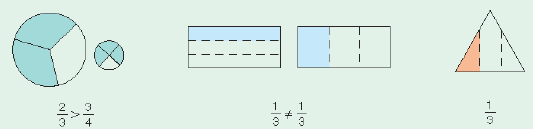
\includegraphics[height=3 cm]{fractionreps}
\end{center}

\fellow{better picture?  this is an old scan from a textbook}

\end{thinkpair*}




\subsection{Units and Unitizing}
In thinking about fractions, it's important to remember that there are always \emph{units} attached to a fraction, even if the units are hidden.  If you see the number $\frac 1 2$ in a problem, you should ask yourself ``half of what?''  The answer to that question is your \emph{unit}, the amount that equals 1.


So far, our units have been consistent: the ``whole'' (or unit) was a whole pie, and fractions were represented by pies cut into equal-sized pieces.  But this is just a model, and we can take anything at all, cut it into equal-sized pieces, and talk about fractions \emph{of that whole}.

One thing that can make fraction problems  so difficult is that the fractions in the problem may be given in different \emph{units} (they may be ``parts'' of different ``wholes'').  




\begin{example}[Everyone is right!]
Mr. Li shows this picture to his class and asks what number is shown by the shaded region.

\begin{center}
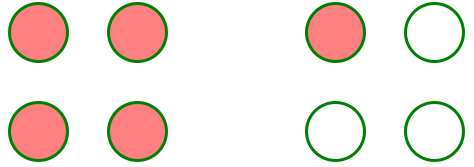
\includegraphics[height = 3cm]{unit1}
\end{center}
\begin{itemize}
\item
Kendra says the shaded region represents the number 5.
\item
Dylan says it represents $2\frac 1 2$.
\item
Kiana says it represents $\frac 5 8$.
\item
Nate says it is $1 \frac 1 4$.
\end{itemize}

Mr. Li exclaims, ``Everyone is right!''

\end{example}

\begin{thinkpair*}\ 
\begin{enumerate}
\item
How can it be that everyone is right?  Justify each answer by explaining what each student thought was the \emph{unit} in Mr. Li's picture.\\

\item
Now look at this picture:
\begin{center}
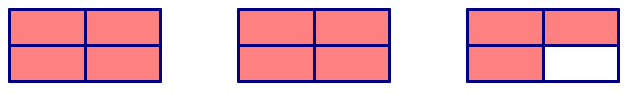
\includegraphics[width = 11cm]{unit2}
\end{center}

\begin{itemize}
\item
If the shaded region represents $3\frac 2 3$, what is the \emph{unit}?
\item
Find three other numbers that could be represented by the shaded region.
\end{itemize}
\end{enumerate}

\end{thinkpair*}



When we think about multiplying fractions, we will (at least at first) choose to think of them as ``portions of line segments,'' since that fits nicely with our  measurement model for numbers.  Then we can once again use an area model to make sense of multiplication.  (We'll do exactly this in the next section!)



\begin{example}[Segments]
  This picture

\includegraphics[height = .5cm]{twothirdsseg}
represents $\frac 2 3$.  The whole segment (the \emph{unit}) is split into three equal pieces by the tick marks, and two of those three equal pieces are shaded.
\end{example}

\begin{thinkpair*}
For each picture below, say what fraction it represents and how you know you're right.

\begin{center}

\includegraphics[width = 3cm]{seg2}
\qquad
\qquad
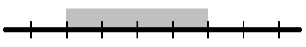
\includegraphics[width = 6cm]{seg3}
\end{center}

\end{thinkpair*}




\subsection{Ordering Fractions}
If we think about fractions as ``portions of a segment,'' then we can talk about their locations on a number line.  We can start to treat fractions like  numbers.  In the back of our minds, we should remember that fractions are always relative to some \emph{unit}.  But on a number line, the unit is clear: it is the distance between 0 and 1.

\fellow{insert picture of number line with the unit distance from 0 to 1 highlighted?}


This measurement model makes it much easier to tackle questions about the relative size of fractions based on where they appear on the number line.  We can mark off different fractions as parts of the unit segment.  Just as with whole numbers, fractions that appear farther to the right are larger.

\fellow{repeat number line, with $3/5$ and $5/8$ marked on it in the correct positions.}


\begin{thinkpair*}[Ordering Fractions]\ 
\begin{enumerate}
\item
What quick method can you use to determine if a fraction is greater than 1?\\

\item
What quick method can you use to determine if a fraction is greater than $\displaystyle \frac 1 2$?\\

\item
Organize these fractions from smallest to largest using \emph{benchmarks}: 0 to $\frac 1 2$, $\frac 1 2$ to 1, and greater than 1, and justify your choices.
\[
\frac{25}{23},\quad  \frac{4}{7}, \quad \frac{17}{35}, \quad \frac{2}{9},  \quad \frac{14}{15}.
\]\\

\item
Arrange each group of fractions in \emph{ascending order}.  Keep track of your thinking and your methods.

\begin{itemize}
\item
$\displaystyle
\frac{7}{17},\quad  \frac{4}{17}, \quad \frac{12}{17}.
$\\

\item
$\displaystyle
\frac{3}{7},\quad  \frac{3}{4}, \quad \frac{3}{8}.
$\\

\item
$\displaystyle
\frac{5}{6},\quad  \frac{7}{8}, \quad \frac{3}{4}.
$\\

\item
$\displaystyle
\frac{8}{13},\quad  \frac{12}{17}, \quad \frac{1}{6}.
$\\


\item
$\displaystyle
\frac{5}{6},\quad  \frac{10}{11}, \quad \frac{2}{3}.
$\\

\end{itemize}

\end{enumerate}



\end{thinkpair*}


You probably came up with benchmarks and intuitive methods to think about the relative sizes of fractions.  Here are some of these methods.  (Did you come up with others?)


\fellow{put the following list in a box with some kind of heading? for the pictures, use the number line model, but shade, for example, the missing pieces when those are discussed }

\noindent
{\bf Greater than 1:} A fraction is greater than 1 if its numerator is greater than the denominator.   How can we see this?  Well, the denominator represents how many pieces in one whole (one unit).  The numerator represents how many pieces in your portion. So if the numerator is bigger, that means you have more than the number of pieces needed to make one whole. \fellow{picture?}  \\


\noindent
{\bf Greater than $\frac 12$:} A fraction is greater than $\frac 1 2$ if the numerator is more than half the denominator.  Another way to check (which might be an easier calculation): a fraction is grater than $\frac 1 2$ if twice the numerator is bigger than the denominator.  Why?  Well, if we double the fraction and get something bigger than 1, then the original fraction must be bigger than $\frac 1 2$.\\

\noindent
{\bf Same denominators:} If two fractions have the same denominator, just compare the numerators. The fractions will be in the same order as the numerators.  For example, $\frac 5 7 < \frac 6 7$.  Why?   Well, the pieces  are the same size since the denominators are the same.  If you have more pieces of the same size, you have a bigger number. \fellow{picture?}  \\

\noindent
{\bf Same numerators: } If the numerators of two fractions are the same, just compare the denominators. The fractions should be in the reverse order of the denominators. For example, $\frac 3 4 > \frac 3 5$.  The justification for this one is a little trickier:  The denominator tells you how many pieces make up one whole.  If there are \emph{more pieces} in a whole (if the denominator is bigger), then the pieces must be \emph{smaller}.  And if you take the same number of pieces (same numerator), then the bigger piece wins.  \fellow{picture?}   \\

\noindent
$\textbf{Numerator} = \textbf{denominator} - 1$: You can easily compare two fractions whose numerators are both one less than their denominators. The fractions will be in the same order as the denominators.  Think of each fraction as a pie with one piece missing. The greater the denominator, the smaller the missing piece,  so the greater the amount remaining. For example, $\frac 6 7 < \frac{10}{11}$, since $\frac 6 7 = 1 - \frac 1 7$ and $\frac {10}{11} = 1 - \frac 1{11}$. \fellow{picture?}  \\


\noindent
$\textbf{Numerator} = \textbf{denominator} - \textbf{constant}$: You can extend the test above to fractions whose numerators are both the same amount less than their denominators. The fractions will again be in the same order as the denominators, for exactly the same reason.  For example, $\frac 3 7 < \frac 7{11}$, because both are  four ``pieces'' less than one whole, and the $\frac 1{11}$ pieces are smaller than the $\frac 17$ pieces. \fellow{picture?}  \\

\noindent
{\bf Equivalent fractions:} Find an equivalent fraction that lets you compare numerators or denominators, and then use one of the above rules. 





\subsection{Arithmetic Sequences}
Consider the patterns below

\begin{align*}
\text{\bf Parttern 1:} &\qquad5, \quad 8, \quad 11, \quad 14, \quad 17, \quad 20, \quad 23, \quad 26, \ldots\\
\text{\bf Parttern 2:} &\qquad2, \quad 9, \quad 16, \quad 23, \quad 30, \quad 37, \quad 44, \quad 51, \ldots\\
\text{\bf Parttern 3:} &\qquad\frac 1 5, \quad \frac 3 5 , \quad 1, \quad \frac 7 5, \quad \frac 9 5, \quad \frac {11}5, \quad \frac {13}5, \quad 3, \ldots
\end{align*}

\begin{thinkpair*}
Answer these questions about each of the patterns.
\begin{enumerate}
\item
Can you predict the next 10 numbers?  \\

\item
Can you predict the 100th number?\\

\item
What do  these sequences have in common?  Describe the pattern in words.
\end{enumerate}


\end{thinkpair*}





The patterns above are called {\bf arithmetic sequences}: a sequence of numbers where the difference between consecutive terms is a constant.  Here are some other examples:
\begin{align*}
\text{\bf Parttern A:} &\qquad\underbrace{1, \quad }_{+1}\underbrace{2, \quad }_{+1}\underbrace{3, \quad }_{+1}\underbrace{4, \quad }_{+1}5, \ldots\\
\text{\bf Parttern B:} &\qquad\underbrace{2, \quad }_{+2}\underbrace{4, \quad }_{+2}\underbrace{6, \quad }_{+2}\underbrace{8, \quad }_{+2}10, \ldots\\
\text{\bf Parttern C:} &\qquad\underbrace{\frac 1 3, \quad}_{+\frac 2 3} \underbrace{ 1 , \phantom{\frac 12}}_{+\frac 2 3}\underbrace{ \frac 5 3, \quad}_{+\frac 2 3}\underbrace{\frac 7 3, \quad}_{+\frac 2 3}  3, \ldots
\end{align*}


\begin{thinkpair*}
If you haven't done so already, find the common difference between terms for Patterns 1, 2, and 3.  Are they really arithmetic sequences?  Then
make up your own arithmetic sequence using whole numbers.  Exchange sequences with a partner, and check if your partner's sequence is really an arithmetic sequence.
\end{thinkpair*}

Here are several more number patterns:
\begin{align*}
\text{\bf Parttern 4:} &\qquad 1, \quad  2 , \quad 4, \quad  8, \quad 16, \quad 32, \quad 64, \quad 128, \ldots\\
\text{\bf Parttern 5:} & \qquad 1, \quad  3 , \quad 6, \quad  10, \quad 15, \quad 21, \quad 28, \quad 36, \ldots\\
\text{\bf Parttern 6:} &\qquad \frac 2 5, \quad \frac 7{10} , \quad 1, \quad \frac {13}{10}, \quad \frac 8 5, \quad \frac {19}{10}, \quad \frac {11}5, \quad \frac 5 2, \ldots\\
\text{\bf Parttern 7:} &\qquad\frac 3 5, \quad \frac 6 5 , \quad \frac {12} 5, \quad \frac {24}{5}, \quad \frac {48} 5, \quad \frac {96}{5}, \ldots
\end{align*}


\begin{thinkpair*}
For each of the sequences above, decide if it is an arithmetic sequence or not.  Justify your answers.
\end{thinkpair*}



\begin{problem}[Fractions in-between]

\[
\frac 1 4, \quad \underline{\qquad}, \quad  \underline{\qquad}, \quad \frac 1 3
\]


\begin{enumerate}
\item
Find two fractions between $\frac 1 4$ and $\frac 1 3$.


\item
Are the resulting four fractions in an arithmetic sequence?  
Justify your answer.
\end{enumerate}


\end{problem}


\begin{problem}[Fractions in-between]
Find two fractions between $\frac 1 6$ and $\frac 1 5$ so the resulting four numbers are in an arithmetic sequence.


\[
\frac 1 6, \quad \underline{\qquad}, \quad  \underline{\qquad}, \quad \frac 1 5
\]



\end{problem}



\begin{problem}[Fractions in-between]
Find three fractions between $\frac 2 5$ and $\frac 5 7$ so the resulting four numbers are in an arithmetic sequence.

\[
\frac 2 5, \quad \underline{\qquad}, \quad \underline{\qquad}, \quad  \underline{\qquad}, \quad \frac 5 7 
\]





\end{problem}


\begin{thinkpair*}[Make your own]
Make up two \emph{fraction} sequences of your own, one that {\bf is} an arithmetic sequence and one that {\bf is not} an arithmetic sequence.  Exchange your sequences with a partner, but don't tell your partner which is which.  When you get your partner's sequences: decide which is an arithmetic sequence and which is not.  Check if you and your partner agree.

\end{thinkpair*}








\section{Multiplying Fractions}

One of our models for  multiplying whole numbers was  an area model. For
example, the product $23\times 37$ is the area (number of $1\times 1 $ squares) of a 23-by-37 rectangle:
\begin{center}
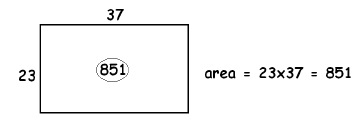
\includegraphics[height = 3cm]{areamodel1}
\end{center}

So the product of two fractions, say, $\frac 4 7 \times \frac 2 3$
should also correspond to an area
problem.


\begin{example}[$\frac 4 7 \times \frac 2 3$]
Let's  start with a  segment of some length that we call 1 unit:
\begin{center}
 
\includegraphics[width = 5cm]{unitseg}
\end{center}
Now, build a square that has one unit on each side:
\begin{center}
 
\includegraphics[width = 5cm]{unitsq}
\end{center}
The area of the square, of course, is $1 \times 1 = 1$ square unit.

Now, let's divide the segment on top into three equal-sized pieces.  (So each piece is $\frac 1 3$.)  And we'll divide the segment on the side into seven equal-sized pieces.  (So each piece is $\frac 1 7$.)
\begin{center}
 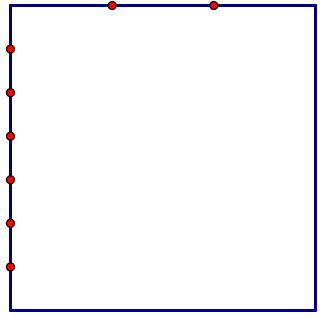
\includegraphics[width = 5cm]{unitsqdiv}
\end{center}
We can use those marks to divide the whole square into small, equal-sized rectangles.  (Each rectangle has one side that measures $\frac 1 3$ and another side that measures $\frac 1 7$.)
\begin{center}
 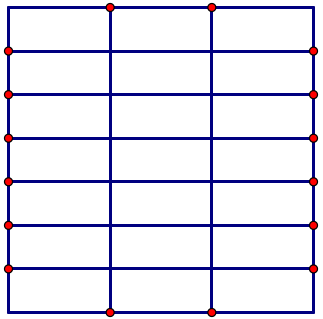
\includegraphics[width = 5cm]{unitsqdiv2}
\end{center}



We can now mark off four sevenths on one side  and two thirds on the other side.
\begin{center}
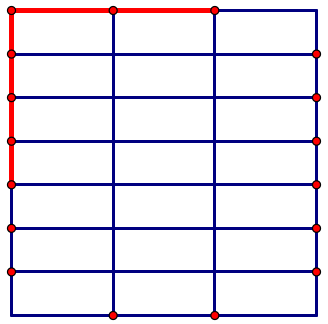
\includegraphics[width = 5cm]{unitsqdiv3}
\end{center}
The result of the multiplication $\frac 4 7 \times \frac 2 3$ should be the area of the rectangle with $\frac 47$ on one side and $\frac 23 $ on the other.  What is that area?
\begin{center}
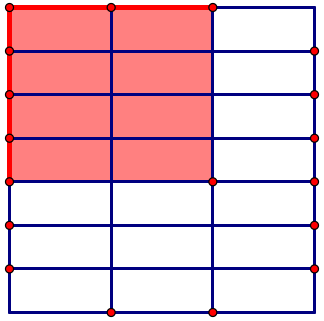
\includegraphics[width = 5cm]{areamodel2}
\end{center}
Remember, the whole square was one-unit.  That one-unit square is divided into 21 equal-sized pieces, and our rectangle (the one with sides $\frac 4 7$ and $\frac 2 3$) contains eight of those rectangles. 
Since the shaded area is the answer to our multiplication problem we conclude that
\[
\frac 47 \times \frac 23 = \frac 8{21}.
\]
\end{example}


\begin{thinkpair*}\ 

\begin{enumerate}
\item
Use this ``unit square method'' to compute each of the following products. 
Draw the picture to
see the answer clearly.
\[
\frac 3 4 \times \frac 5 6,
\qquad\qquad\qquad
\frac 3 8 \times \frac 5{10},
\qquad\qquad\qquad
\frac 5 8 \times \frac 3 7 .
\]\\

\item
The area problem $\frac 4 7 \times \frac 2 3$
yielded a diagram with 21 small rectangles. 
Explain \emph{why} 21 appears as the total number of equal-sized rectangles.\\


\item
The area problem $\frac 4 7 \times \frac 2 3$
yielded a diagram with 8 small shaded rectangles. 
Explain \emph{why} 8 appears as the number of shaded rectangles\\
\end{enumerate}

\end{thinkpair*}


\begin{problem}[Extend the Model]
How can you extend the area model for fractions greater than 1?  Try to draw a picture for each of these:

\[
\frac 3 4 \cdot \frac 3 2,
\qquad \qquad\qquad
\frac 2 5 \cdot \frac 4 3,
\qquad \qquad\qquad
\frac 3 {10} \cdot \frac 5 4,
\qquad \qquad\qquad
\frac 5 2 \cdot \frac 7 4.
\]

\end{problem}





\subsection*{On Your Own} 
Work on the following exercises on your own or with a partner.

\begin{enumerate}
\item
Compute the following products, simplifying each of the answers as
much as possible.  You do not need to draw pictures, but you may certainly choose to do so if it helps! 
\[
\frac 5{11} \times \frac 7{12},
\qquad\qquad
\frac 4 7 \times \frac 4 8,
\qquad\qquad
\frac 1 2 \times \frac 1 3,
\qquad\qquad
\frac 2 1 \times \frac 3 1,
\qquad\qquad
\frac 15 \times \frac 51.
\]\\

\item
Compute the following products.  (Don't work too hard!)

\[
\frac 3 4 \times \frac 1 3 \times \frac 2 5,
\qquad\qquad
\frac 5 5 \times \frac 7 8 ,
\qquad\qquad
\frac{88}{88} \times \frac{541}{788},
\qquad\qquad
\frac{77876}{311} \times \frac{311}{77876}.
\]\\

\item
Try this one.  Can you make use of the fraction rule $\frac{xa}{xb} = \frac a b$ to help you calculate?  How?
\[
\frac 1 2 \times \frac 23 \times \frac 34 \times \frac 45 \times \frac 56\times \frac 67 \times \frac 78 \times\frac 89 \times
\frac9{10}
\]\\

\end{enumerate}


You probably simplified your work in the exercises above by using a multiplication rule like the following.

\fellow{put the rule a box, centered?}

{\bf Multiplying Fractions:}
\[
\frac a b \cdot \frac cd 
\quad
=
\quad
 \frac{a\cdot c}{b\cdot d}.
\]

Of course, you may then choose to simplify the final answer, but the answer is always \emph{equivalent} to this one.  Why?  The area model can help us explain what's going on.  

First, let's clearly write out how the area model says to multiply $\frac ab \cdot \frac cd$.  We want to build a rectangle where one side has length $\frac a b$ and the other side has length $\frac c d$.  We start with a square, one unit on each side.
\begin{itemize}
\item
Divide the top segment into $b$ equal-sized pieces.  Shade $a$ of those pieces.  (This will be the side of the rectangle with length $\frac a b$.)\\

\item
Divide the left segment into $d$ equal-sized pieces.  Shade $c$ of those pieces.  (This will be the side of the rectangle with length $\frac c d$.)\\

\item
Divide the whole rectangle according to the tick marks on the sides, making equal-sized rectangles.\\

\item
Shade the rectangle bounded by the shaded segments.\\

\end{itemize}

\fellow{add an animation of this process in a couple of examples?}


If the answer is $\frac{a\cdot c}{b\cdot d}$, that means there are $b\cdot d$ total equal-sized pieces in the square, and $a\cdot c$ of them are shaded.  We can see from the model why this is the case:

\begin{itemize}
\item
The top segment was divided into $b$ equal-sized pieces.  So there are $b$ columns in the rectangle.\\

\item
The side segment was divided into $d$ equal-sized pieces.  So there are $d$ rows in the rectangle.\\

\item
A rectangle with $b$ columns and $d$ rows has $b\cdot d$ pieces.  (This is exactly our area model for whole-number multiplication!)\\
\end{itemize}

\begin{thinkpair*}
Stick with the general multiplication rule
\[
\frac a b \cdot \frac cd = \frac{a\cdot c}{b\cdot d}.
\]
With a partner, write a clear explanation for why $a\cdot c$ of the small rectangles will be shaded.

\end{thinkpair*}







\subsection{Multiplying Fractions by Whole Numbers}
Often, elementary students are taught to multiply fractions by whole numbers using the fraction rule.

\begin{example}[$2 \cdot \frac 3 7$, Multiply Fractions]
For example, to multiply  $2 \cdot \frac 3 7$, we think of ``2'' as $\frac 2 1$, and compute this way:
\[
2 \cdot \frac 37 
\quad
= 
\quad
\frac 21 \cdot \frac 37 
\quad
= 
\quad
\frac{2\cdot3}{1\cdot7}
\quad
 = 
 \quad
 \frac 67.
\]
\end{example}


We can also think in terms of our original ``Pies Per Boy Model'' to answer questions like this.

\begin{example}[$2 \cdot \frac 3 7$, Pies Per Boy]
We know that $\frac 3 7$ means the amount of pie each boy gets when 7 boys evenly share 3 pies.

If we compute $2\cdot \frac 37$, that means we double the amount of pie each boy gets.  We can do this by doubling the number of pies.  So the answer is the same as $\frac 67$: the amount of pie each boy gets when 7 boys evenly share 6 pies.
\end{example}


Finally, we can think in terms of units and unitizing.

\begin{example}[$2 \cdot \frac 3 7$, Units]
The fraction $\frac 3 7$ means that I have 7 equal pieces (of \emph{something}), and I take 3 of them.

So $2\cdot \frac 37$ means do that twice.  If I take 3 pieces and then 3 pieces again, I get a total of 6 pieces.  There are still 7 total pieces, so the answer is $\frac 6 7$.

\end{example}


\begin{thinkpair*}\ 
\begin{enumerate}
\item
Use all three methods to explain how to find each product:
\[
3 \cdot \frac 2 5 ,
\qquad\qquad\qquad
4 \cdot \frac 3 8 ,
\qquad\qquad\qquad
6 \cdot \frac 1 5.
\]

\item
Compare these different ways of thinking about fraction multiplication.  Are any of them more natural to you?  Does one make more sense than the others?  Do the particular numbers in the problem affect your answer?  Does your partner agree?
\end{enumerate}
\end{thinkpair*}


Let's think so more about the expression 
\[
4 \cdot \frac 38.
\]
Using the first method (multiplying fractions), we compute:
\[
4 \cdot \frac 38 
\quad
=
\quad
 \frac 41 \cdot \frac 38
 \quad
  = 
  \quad
  \frac{12}8.
\]
And we might notice that this simplifies:
\[
\frac{12}8 
\quad
=
\quad
 \frac{3\cdot 4}{2\cdot 4} 
 \quad
 = 
 \quad
 \frac 32.
\]

Here's another example:
\[
10 \cdot \frac 2{15} 
\quad
=
\quad
 \frac{10} 1 \cdot \frac 2{15} 
\quad
= 
\quad
\frac{10\cdot 2}{15}.
\]
Rather than multiply out the numerator, let's break everything down as far as we can into factors:
\[
 \frac{10\cdot 2}{15} 
 \quad
=
\quad
\frac{2\cdot 5 \cdot 2}{3\cdot 5}
\quad
=
\quad
 \frac{2\cdot2}{3} 
 \quad
=
\quad
\frac{4}{3}.
\]



Here's one more example:
\[
8 \cdot \frac{212}{16} 
\quad
= 
\quad
\frac{8 \cdot 212}{16}.
\]
We can avoid some work (mathematicians \emph{love} to avoid work and make things easier on themselves!) if we notice that $16 = 8 \cdot 2$:
\[
8 \cdot \frac{212}{16} 
\quad
=
\quad
 \frac{8 \cdot 212}{8\cdot 2} 
 \quad
 =
 \quad
  \frac{212}{2}
  \quad
   = 
   \quad
   106.
\]

\subsection*{On Your Own}
Try these exercises on your own or with a partner.

\begin{enumerate}
\item
Compute each of the following and write your answer in simplified form.  Avoid doing extra work if you can!
\[
17 \cdot \frac 2 3,
\qquad\qquad
10 \cdot \frac 1 5 ,
\qquad\qquad
\frac 3 4 \cdot 4,
\qquad\qquad
11 \cdot \frac{36}{33},
\qquad\qquad
\frac{13}{12} \cdot 24.
\]

\item
Compute each of the following and write your answer in simplified form.  Look for shortcuts!
\[
\frac 3 7 \cdot \frac 7 5,
\qquad\qquad
\frac{133}{112} \cdot 224,
\qquad\qquad
\frac{39}{35}\cdot\frac{14}{13},
\qquad\qquad
\frac 5{13} \cdot \frac 47 \cdot \frac{13}2  \cdot \frac 7{10}.
\]
\end{enumerate}

\begin{thinkpair*}\ 
\begin{enumerate}
\item
Compute the following:
\[
6 \cdot \frac 5 6,
\qquad\qquad\qquad
\frac{7}{18} \cdot 18.
\]\\

\item
What can you say about these products?  Carefully justify your answer using (at least) one of the models for multiplication above.
\[
b \cdot \frac a b,
\qquad\qquad\qquad
\frac cd \cdot d.
\]\\

\item
Keo was asked to compute
\[ 
\frac{18}7 \cdot \frac{70}{36}.
\]
Within three seconds, he shouted ``The answer is 5!''  Is he right?  How was he able to compute it so quickly?\\
\end{enumerate}
\end{thinkpair*}


Roy says that the fraction rule
\[
\frac{xa}{xb} = \frac ab
\]
is ``obvious'' if
you think in terms of multiplying fractions. He reasons as follows:

\begin{quotation}
\emph{
We know multiplying anything by 1 doesn't change a number:
\begin{align*}
1 \cdot 4 &= 4\\
1 \cdot 2014 &= 2014\\
1 \cdot \frac 5 7 &= \frac 5 7.
\end{align*}
So in general
\[
1 \cdot \frac a b = \frac a b.
\]
Now, $\frac 2 2 = 1$, so that means that 
\begin{align*}
\frac 2 2 \cdot \frac a b &= \frac a b, \text{ which means}\\
\frac{2a}{2b} &= \frac a b.
\end{align*}
By the same reasoning, $\frac 3 3  = 1$, so that means that 
\begin{align*}
\frac 3 3 \cdot \frac a b &= \frac a b, \text{ which means}\\
\frac{3a}{3b} &= \frac a b.
\end{align*}
}
\end{quotation}


\begin{thinkpair*}
What do you think about Roy's reasoning?  Does it make sense?
How would Roy explain the general rule for positive whole numbers $x$:
\[
\frac{xa}{xb} = \frac a b?
\]
\end{thinkpair*}




\subsection{Fractions of fractions of fractions of fractions of\dots}
\begin{thinkpair*}
How are these two problems different?  Draw a picture of each.
\begin{enumerate}
\item
Pam had $\frac 2 3$ of a cake in her refrigerator, and she ate half of it.  How much total cake did she eat?
\item
On Monday, Pam ate $\frac 2 3$ of a cake.  On Tuesday, Pam at $\frac 1 2$ of a cake.  How much total cake did she eat?
\end{enumerate}
\end{thinkpair*}




When a problem includes a phrase like ``$\frac 2 3 $ of \dots,'' students are taught to treat ``of'' as multiplication, and to use that to solve the problem.  As the above problems show, in some cases this makes sense, and in some cases it does not.  It's important  to read carefully and understand what a problem is asking, not memorize rules about ``translating'' word problems.

If I have 12 circles and I want ``$\frac 2 3$ of the circles,'' I can take two out of every three cirlces.
\fellow{ add a picture: 12 circles, divided into three groups, with two shaded from each group}

  I can also take $\frac 2 3$ from each individual circle.  
  \fellow{ add a picture of 12 circles, each divided into thirds with 2/3 shaded}
  
  In both cases, I can compute the answer as 
 $\frac 2 3 \times 12$ circles, but the reasoning in each case is a little different.  
 
 In the first case, we are really thinking of ``$\frac 2 3$ of 12'' as a sequence of operations: 
 \begin{itemize}
 \item
 Divide my 12 circles groups of three circles each.  
 \item
 Shade 2 circles in every group.  
 \end{itemize}
 So I have computed this way:
 \[
 (12 \div 3) \cdot 2 
 \quad
 =
 \quad
 \frac{12}3 \cdot 2 
 \quad
 =
 \quad
 \frac{12\cdot 2}{3}
 \quad
 =
 \quad
 12 \cdot \frac 2 3.
 \]
 
 In the second case, we are really think of $\frac 2 3$ of a circle, repeated 12 times, which is also
 \[
 \frac 2 3 \cdot 12.
 \]

If we change the numbers, sometimes one of the interpretations is more natural than the other.  For example, how can we understand ``$\frac 3 5$ of 12''?  We can interpret this as ``take 3 of every 5 circles,'' but this doesn't really make sense because we can't divide 12 circles into groups of 5 circles each.  It's easier to take $\frac 3 5$ of each circle.

\fellow{add picture?}


\begin{thinkpair*}\ 
\begin{enumerate}
\item
Draw $\frac 5 8$ of 4 circles in two different ways.  What is $\frac 5 8$ of 4?\\
\item
 Draw $\frac 3 4$ of 2 candy bars in two different ways.  What is $\frac 3 4$ of 2?\\
 \item
 Draw a rectangle and shade $\frac 2 3$ of $\frac 3 4$ of the rectangle.  What is $\frac 23 \cdot \frac 3 4$?\
 \end{enumerate}

\end{thinkpair*}






\section{Dividing Fractions: Meaning}
We had several ways to think about division of whole numbers:
\begin{itemize}
\item
{\bf Quotatitive model:} Make groups of a given size.  For example, for $18 \div 3$, we start with 18 dots (or candy bars or molecules), and we make groups of 3 dots (or 3 whatevers).  We ask: how many groups can we make?\\

\item
{\bf Partitive model:} Make a given number of groups.  For $18 \div 3$, we say start with 18 dots (or people or pencils), and we make three equal-sized groups.  We ask: how many objects are in each group?\\

\item
{\bf Missing factor model:} Solve a multiplication problem instead.  For $18 \div 3$, we rewrite the problem as $3 \cdot \underline{\qquad} = 18$.\\
\end{itemize}

We can still think about all of these models when we divide fractions, but actually doing the calculation can be tricky!

\begin{thinkpair*}\label{partorquot}
For each problem below, draw a picture of the situation, and  label the problem as partitive or quotative.  Explain your thinking.  Then try to solve each of the problems.  Find as many different ways as you can to justify your solutions.


\begin{enumerate}
\item
It took Mary four bucketfuls of water to fill up her three gallon fish tank.  How much water does her bucket hold?\\

\item
You have $\frac 2 3$ of a gallon of water in a bucket, and the bucket is $\frac 7 8$ full.  How many gallons would it take to fill up the whole bucket?\\


\item 
$10\frac 1 2$ gallons of water fills up $2 \frac 1 3$ buckets.  How many gallons are in one bucket?\\

\item
Mr. Brown has a length of rope that measures $10 \frac 1 2$ yards long.  Each boy in his scout troop needs a piece $2 \frac 1 3$ yards long.  How many pieces of the required length can he cut?\\


\end{enumerate}



\end{thinkpair*}




Most people find problem (2) above quite challenging, and have a hard time both drawing a picture and being certain they have the right answer.  (Even if you didn't find it so difficult, certainly you can imagine that some of your future students would be stumped by such a problem!)  

If a problem is giving us trouble, what are some things we can do?  Solve a simpler problem!
Let's rephrase problem (2) in several new ways:
\begin{enumerate}[(2a)]
\item
You have $\frac 2 3$ of a gallon of water in a bucket, which fills up $\frac 1 2$ of your bucket.  How many gallons total would it take to fill up the whole bucket?\\

\item
You have $\frac 2 3$ of a gallon of water in a bucket, which fills up $\frac 1 3$ of your bucket.  How many gallons total would it take to fill up the whole bucket?\\

\item
You have $\frac 2 3$ of a gallon of water in a bucket, which fills up $\frac 1 4$ of your bucket.  How many gallons total would it take to fill up the whole bucket?\\

\item
You have $\frac 2 3$ of a gallon of water in a bucket, which fills up $\frac 1 5$ of your bucket.  How many gallons total would it take to fill up the whole bucket?\\

\item
 You have $\frac 2 3$ of a gallon of water in a bucket, which fills up $\frac 1 8$ of your bucket.  How many gallons total would it take to fill up the whole bucket?\\

\end{enumerate}

\begin{thinkpair*}
Each of the problems above is significantly easier than the original problem (2).  Discuss with a partner why these questions are easier.  For each one, draw a picture and find the solution.  Most importantly, find a general method to answer this question:

\begin{quotation}
\emph{
If $\frac 2 3$ of a gallon  of water fills my bucket to the $\frac 1 n$ mark, how much water does my bucket hold?}
\end{quotation}
\end{thinkpair*}


So, back to original problem --- what's complicated in that case?  The water doesn't fill your bucket to the $\frac 1 8$ mark.  It fills your bucket to  the $\frac 7 8$ mark.
Here are some helpful questions to think about the next step of the problem:
\begin{enumerate}[(2a')]

\item
You have $\frac 2 3$ of a gallon of water in a bucket, which fills up $\frac 3 4$ of your bucket.  How many gallons  would it take to fill up $\frac 1 4$ of the bucket?  How many total to fill up the whole bucket?\\


\item
You have $\frac 2 3$ of a gallon of water in a bucket, which fills up $\frac 3 5$ of your bucket.  How many gallons  would it take to fill up $\frac 1 5$ of the bucket?  How many total to fill up the whole bucket?\\

\item
 You have $\frac 2 3$ of a gallon of water in a bucket, which fills up $\frac 5 8 $ of your bucket.  How many gallons  would it take to fill up $\frac 1 8$ of the bucket?  How many total to fill up the whole bucket?\\

\end{enumerate}


\begin{thinkpair*}
Work on the questions above with a partner.  Your goal is to be able to answer this question:

\begin{quotation}
\emph{If  $\frac 2 3$ gallons of water fills my bucket to the $\frac a b$ mark, how can I find the total number of gallons that fills my bucket to the $\frac 1 b$ mark?}
\end{quotation}

If you can answer that, you should be able to apply it to answer the original version of problem (2) above.
\end{thinkpair*}







\section{Dividing Fractions: Computations}

All of the following questions have the same answer!  (Why?)
\begin{itemize}
\item
How many groups of 3 are there in 6?
\item
How many groups of 3 tens are there in 6 tens?
\item
How many groups of 3 fives are there in 6 fives?
\item
How many groups of 3 tenths are there in 6 tenths?
\item
How many groups of 3 fourths are there in 6 fourths?
\item
How many groups of 3 @s are there in 6 @s?
\item
How many groups of 3 anythings are there in 6 anythings (as long as both ``anythings'' refer to the same unit)?
\end{itemize}



\begin{thinkpair*}
With a partner, draw some pictures to illustrate each of the questions above.  Do you believe that they all have the same answer?  Use a picture or reasoning to solve each of the following fraction division problems:

\[
\frac 6 4 \div \frac 3 4,
\qquad\qquad
\frac 6{10} \div \frac 3{10},
\qquad\qquad
\frac 8 9 \div \frac 4 9,
\qquad\qquad
\frac{15}{33} \div \frac{1}{33},
\qquad\qquad
\frac{10}9 \div \frac{5}9.
\]

\end{thinkpair*}

\subsection{Common denominator method}
This line of reasoning leads  to our first fraction division method.  
If two fractions have the same denominator, then when you divide them, you can just divide the numerators.  In symbols,

\[
\frac a d \div \frac b d = \frac a b.
\]


\begin{thinkpair*}
What if the fractions \emph{don't} have a common denominator?  Is the method useless, or can you find a way to make it work?  Can you solve these problems?

\[
\frac 3 5 \div \frac 3 4,
\qquad\qquad\qquad
\frac 3 4  \div \frac 8 7,
\qquad\qquad\qquad
\frac 2 3  \div \frac 1 2,
\qquad\qquad\qquad
\frac 5 8  \div \frac 1 4.
\]
\end{thinkpair*}




\subsection{Missing factor approach}
We know that we can always turn a division problem into a ``missing factor'' multiplication problem.  Can that help us compute fraction division?  Sometimes!

\begin{thinkpair*}
For each division problem, rewrite it as a missing factor multiplication question.  Then answer that  question using what you know about multiplying fractions.

\[
\frac{9}{10} \div \frac{3}{5},
\qquad\qquad
\frac 7 8  \div \frac 1 4,
\qquad\qquad
\frac 6 7  \div \frac 3 7,
\qquad\qquad
\frac{10}9 \div \frac 2 3,
\qquad\qquad
\frac{25}{12} \div \frac 5 6.
\]


\end{thinkpair*}


\subsection*{A nasty problem:}

\begin{quotation}
\emph{$7\frac 2 3$ 
pies are  shared equally by $5\frac 34$ boys.
 How much pie does each boy get?
} \end{quotation}


Technically, we could just write down the answer as
\[
\frac{7\frac 2 3}{5\frac 34}
\]
and be done! (The answer to this problem is, of course, equivalent to this fraction, so why not?) 

Is there a way to make this look
friendlier?
Recall the key fraction rule:
\[
\frac{xa}{xb} = \frac a b.
\]

What might happen if we multiply the numerator and denominator of our answer each by a convenient
choice of number? Right now we have the expression:
\[
\frac{7\frac 2 3}{5\frac 34}
\quad
=
\quad
\frac{\left(7+\frac 2 3\right)}{\left(5+ \frac 34\right)}.
\]

Let's multiply by 3. (Why three?)
\[
\frac{\left(7+\frac 2 3\right)\cdot 3}{\left(5+ \frac 34\right)\cdot 3}
\quad
=
\quad
\frac{\left(21+2\right)}{\left(15+ \frac 94\right)}.
\]
{\bf Important Note:} We're using some key facts about arithmetic here!  First, we used the distributive law for multiplication over addition: 
\[
(a+b)\cdot c 
\quad
= 
\quad
a\cdot c + b\cdot c. \qquad \text{(Where have we used this fact?) }
\]   Second, we used what we know about multiplying fractions by whole numbers.  In particular, we used the fact that 
\[
\frac a b \cdot b
\quad
 = 
 \quad
 a.\qquad  \text{(Where did we use that fact?)}
\]

Let's now multiply numerator and denominator each by 4. (Why four?)
\[
\frac{\left(21+2\right)\cdot 4}{\left(15+ \frac 94\right)\cdot 4}
\quad
=
\quad
\frac{84+8}{60+9} 
\quad
= 
\quad
\frac{92}{69}.
\]

We now see that the answer is $\frac{92}{69}$.  That means that sharing $7\frac 2 3$ 
pies among $5 \frac 3 4$ boys
 is the same as
sharing 92 pies among 69 boys.  (That is, in both situations, the individual boys get exactly the same amount of pie.)


\begin{example}
Let's forget the context now and just focus on the calculations so that we can see what's going on more clearly.  Try this one:
\[
\frac{3\frac 12}{1\frac 1 2}.
\]
Multiplying the numerator and denominator each by 2 should be enough to simplify
the expression.  (Why?)  Let's try it:
\[
\frac{3\frac 12}{1\frac 1 2}
\quad
=
\quad
\frac{3+\frac 12}{1+\frac 1 2}
\quad
=
\quad
\frac{\left(3+\frac 12\right)\cdot 2}{\left(1+\frac 1 2\right)\cdot 2}
\quad
=
\quad
\frac{6+1}{2+1} 
\quad
= 
\quad
\frac 73.
\]



\end{example}

\subsection*{On Your Own}
Each of the following is a perfectly nice fraction, but it could be written in a simpler form.  So do that!  Write each of them in a simpler form following the examples above.

\[
\frac{4\frac 2 3}{5 \frac 1 3},
\qquad\qquad\qquad
\frac{2 \frac 15}{2 \frac 14},
\qquad\qquad\qquad
\frac{1\frac 47}{2\frac 3{10}},
\qquad\qquad\qquad
\frac{\frac37}{\frac45}.
\]

\begin{thinkpair*}\ 
\begin{enumerate}
\item
Jessica calculated the second exercise above this way:
\[
\frac{2 \frac 15}{2 \frac 14} 
\quad
=
\quad
\frac{\cancel{2} \frac 15}{\cancel{2} \frac 14}
\quad
=
\quad
\frac{\frac 15}{\frac 14}
\quad
 =
 \quad
\frac{\frac 15 \cdot 4}{\frac 14\cdot 4}
\quad
 = 
 \quad
\frac{\frac 45}{1}
\quad
 =
 \quad
  \frac 45.
\]
Is her solution correct, or is she misunderstanding something?  Carefully explain what's going on with her solution, and what you would do as Jessica's teacher.\\

\item
Isaac calculated the last exercise above this way:
\[
\frac{\frac37}{\frac45}
\quad
=
\quad
\frac{\frac37\cdot 7}{\frac45 \cdot 5}
\quad
=
\quad
\frac 34.
\]
Is his solution correct, or is he misunderstanding something?  Carefully explain what's going on with his solution, and what you would do as Isaac's teacher.

\end{enumerate}

\end{thinkpair*}


\subsection{Simplify an ugly fraction!}
Perhaps without realizing it, you have just found another method to divide fractions.

\begin{example}[$\frac 35 \div \frac 47$]
Suppose we are  asked about sharing $\frac 3 5$
of a pie among $\frac 4 7$
of a boy (whatever that would mean!). That is,
we are  asked to compute:
\[
\frac{\frac 3 5}{\frac 4 7}.
\]
Let's multiply numerator and denominator each by 5:
\[
\frac{\left(\frac 3 5\right)\cdot5}{\left(\frac 4 7\right)\cdot 5}
\quad
=
\quad
\frac{3}{\frac{20}7}.
\]
Let's now multiply top and bottom each by 7:
\[
\frac{\left(3\right)\cdot 7}{\left(\frac{20}7\right)\cdot 7}
\quad
= 
\quad
\frac{21}{20}.
\]
Done!  So $\frac 3 5 \div \frac 4 7 = \frac {21}{20}$.
\end{example}


\begin{example}[$\frac 5 9 \div \frac 8{11}$]
Let's do another. Consider $\frac 5 9 \div \frac 8{11}$:
\[
\frac{\frac 59}{\frac 8{11}}
\]
Let's multiply top and bottom each by 9 and by 11 at the same time. (Why not?)
\[
\frac{\frac 59}{\frac 8{11}}
\quad
 =
 \quad
\frac{\left(\frac 59\right)\cdot9\cdot 11}{\left(\frac 8{11}\right) \cdot 9\cdot 11}
\quad
= 
\quad
\frac{5\cdot 11}{8\cdot 9}.
\]
(Do you see what happened here?)

So we have 
\[
\frac{\frac 59}{\frac 8{11}}
\quad
=
\quad
\frac{5\cdot 11}{8\cdot9}
\quad
 = 
 \quad
 \frac {55}{72}.
\]
\end{example}



\subsection*{On Your Own}
Compute each of the following, using the simplification technique.
\[
\frac 12 \div \frac 1 3,
\qquad\qquad
\frac 4 5 \div \frac 3 7,
\qquad\qquad
\frac 2 3 \div \frac 1 5,
\qquad\qquad
\frac {45}{59} \div \frac {902}{902},
\qquad\qquad
\frac{10}{13} \div \frac{2}{13}.
\]



\subsection{Invert and multiply}
Consider the problem
$\frac 5 {12} \div \frac 7 {11}$.
Janine wrote:
\[
\frac{\frac 5 {12} }{ \frac 7 {11}} 
\quad
= 
\quad
\frac{\frac 5 {12} \cdot 12\cdot 11}{ \frac 7 {11} \cdot 12 \cdot 11} 
\quad
= 
\quad
\frac{ 5 \cdot 11 }{  7\cdot 12} 
\quad
=
\quad
\frac 5{12} \cdot \frac{11} 7.
\]
She stopped before completing her final step and  exclaimed: 
``Dividing one fraction by another is the same as multiplying
the first fraction with the second fraction upside down.''


\subsection*{On Your Own}
First check each step of Janine's work here and make sure that she is correct in what
she did up to this point.  Then answer these questions:
\begin{enumerate}
\item
Do you understand what Janine is saying?  Explain it very clearly.\\


\item
Work out
\[
\frac{\frac{3}{7}}{\frac4{13}}
\]
using the simplification method.  Is the answer the same as
$\frac 3 7 \cdot \frac{13}4$?\\

\item
Work out
\[
\frac{\frac{2}{5}}{\frac 3{10}}
\]
using the simplification method.  Is the answer the same as
$\frac 2 5 \cdot \frac{10}3$?\\

\item
Work out
\[
\frac{\frac{a}{b}}{\frac c{d}}.
\]
using the simplification method.  Is the answer the same as
$\frac a b \cdot \frac{d}c$?\\

\item
Is Janine right? Is dividing two fractions always the same as multiplying the
two fractions with the second one turned upside down? What do you think?  (Don't just think about  examples.  This is a question if something is \emph{always} true.)\\

\end{enumerate}


We now have several methods for solving problems that require dividing fractions:

\fellow{Put this in a box?}

\noindent
{\bf Dividing fractions:}
\begin{enumerate}
\item
Find a common denominator and divide the numerators.
\item
Rewrite the division as  a missing factor multiplication problem, and solve that problem.
\item
Simplify an ugly fraction.
\item
Invert the second fraction (the dividend) and then multiply.

\end{enumerate}


\begin{thinkpair*}
Discuss your opinions about our four methods for solving fraction division problems with a partner:

\begin{itemize}
\item
Which method for division of fractions is the easiest to \emph{understand why it works}? 
\item
Which method for division of fractions is the easiest to \emph{use in computations}? 
\item
What are the benefits and drawbacks of each method?  (Think both as a teacher and as someone solving math problems here.) 
\end{itemize}
\end{thinkpair*}




\section{Fraction Sense}

\begin{thinkpair*}
For each of the following problems, suppose $a$ and $b$ are both fractions that are between $0$ and $1$, and suppose $a$ is bigger than $b$.  Decide which symbol should go in the $\square$ for each equation: $>$, $<$,  or $=$.  Justify your answer, and keep in mind that more than one symbol may be possible!

\begin{enumerate}
\item
Addition:
\[
a + b \quad  \square \quad a,
\qquad\qquad
a + b \quad  \square \quad b,
\qquad\qquad
a + b \quad  \square \quad 0
\qquad\qquad
a + b \quad  \square \quad 1.
\]\\

\item
Subtraction:
\[
a - b \quad  \square \quad a,
\qquad\qquad
a - b \quad  \square \quad b,
\qquad\qquad
a - b \quad  \square \quad 0
\qquad\qquad
a - b \quad  \square \quad 1.
\]\\


\item
Multiplication:
\[
a\cdot b \quad  \square \quad a,
\qquad\qquad
a \cdot b \quad  \square \quad b,
\qquad\qquad
a \cdot b \quad  \square \quad 0
\qquad\qquad
a \cdot b \quad  \square \quad 1.
\]\\



\item
Division:
\[
a\div b \quad  \square \quad a,
\qquad\qquad
a \div b \quad  \square \quad b,
\qquad\qquad
a \div b \quad  \square \quad 0
\qquad\qquad
a \div b \quad  \square \quad 1.
\]\\


\end{enumerate}
\end{thinkpair*}


\subsection{Multiplying and Dividing}
Elementary school students are often taught mental shortcuts like ``multiplication makes things bigger.''  But is that necessarily true?  You have to be careful as a teacher to make ideas simple for students to understand, but not so simple that you say things that are wrong!

Let's try some examples.

\begin{example}[Multiplying by $\frac 5 4$]
Let's try it with 100:
\[
\frac 5 4 \cdot 100 
\quad
= 
\quad
\frac{500}4 
\quad
= 
\quad
125.
\]
Yep, that's bigger than 100.  
\end{example}

But of course this is only one example.  How can we be sure that multiplying \emph{any}  (positive)  number by $\frac 5 4$ gives a result that's bigger than that number?  That is, how can we be sure that
\[
\frac 5 4 \cdot X
\quad
 > 
 \quad
 X \qquad \text{ for every choice of } X?
\]
This is a \emph{universal} statement, so one example is not enough to be sure it's true.  We need an explanation!  And here it is.

We can rewrite $\frac 54$ as $1 + \frac 14$.  So then
\[
\frac 5 4 \cdot X 
\quad
=
\quad
\left(1 + \frac 1 4\right)\cdot X
\quad
=
\quad
X + \frac 1 4 \cdot X 
\quad 
=
\quad
X + \text{ more }.
\]
So the answer is bigger than $X$.

\begin{thinkpair*}
Go through each step in the series of calculations above, and explain what is going on.  Where is the distributive law used?  Where do we need the fact that $X$ is a positive number?  Then:
\begin{enumerate}
\item
Write a careful argument that multiplying a (positive) number by $\frac 8 5$ gives a result that is larger than the original number.\\
\item
 Write a careful argument that multiplying a (positive) number by $\frac {20} 9$ gives a result that is larger than the original number.\\
 \end{enumerate}

\end{thinkpair*}

Does this rule hold for other fractions as well?  Does multiplication always result in a larger number than the one being multiplied?  Let's try another example.

\begin{example}[Multiplying by $\frac 4 5$]
  Again, we'll use 100 as our first test case:
\[
\frac 4 5 \cdot 100 = \frac{400} 5 = 80.
\]
So in this case, the result is \emph{smaller} than 100!  
\end{example}

This counterexample shows that the following  universal statement is {\bf definitely false}:
\emph{Multiplying a positive number $X$ by $\frac 4 5$ gives a result that is bigger than $X$.}


We might ask the following:
\begin{center}
\emph{Is it always true that  $\frac 4 5 \cdot X < X$ for a positive number $X$?}
\end{center}

Notice, this is not the same question!  We know that the answer is not \emph{always} bigger than $X$.  But we don't know it it is \emph{always} smaller.  It could be \emph{sometimes} bigger and \emph{sometimes} smaller.  How can we be sure?

You might have already guessed what to do.  We thought about $\frac 5 4$ as ``one plus a little bit.''  In a very similar way, we can think about $\frac 4 5$ as ``a little bit less than one,'' and use that to explain why, indeed, the result must always be smaller.  Here we go:

Notice that $\frac 4 5 = 1 - \frac 1 5$.  So we can write
\[
\frac 4 5 \cdot X 
\quad
=
\quad
\left( 1 - \frac 1 5\right) \cdot X
\quad 
=
\quad
X - \frac 1 5\cdot X
\quad
=
\quad
X - \text{some smallish amount},
\]
and the result will be smaller than $X$.

\begin{thinkpair*}
Go through each step in the series of calculations above, and explain what is going on.  Where is the distributive law used?  Where do we need the fact that $X$ is a positive number?  Then:
\begin{enumerate}
\item
Write a careful argument that multiplying a (positive) number by $\frac 7 8$ gives a result that is smaller than the original number.\\
\item
 Write a careful argument that multiplying a (positive) number by $\frac 5 9$ gives a result that is smaller than the original number.\\
 \end{enumerate}

\end{thinkpair*}

It may seem silly to write such careful arguments for things you already know to be true.  Of course multiplying by a number less than one makes your answer smaller!

Well, let's make two comments:
\begin{itemize}
\item
The fact that this is obvious to you (if it is!) comes from your years of experience with numbers.  When students first learn about fractions, it is ``obvious'' to them that multiplying makes things bigger.  In their experience, it has always done so!  Our intuition is based on our experiences, and cannot always be trusted!  That's why explanation and justification play such a crucial role in mathematics.
\item
Though many people think the results are obvious when dealing with multiplication, they can get completely turned upside down (so to speak) in dealing with division.  And it always helps to work through the relatively simple case first, before tackling the more difficult one.
\end{itemize}


\noindent{\bf Claim:} If we divide a positive number by some fraction less than one, the result is \emph{bigger} than the original number.

Before trying to justify a claim, we should always check a few examples to see if we even believe that it's true.  Testing these ideas out on the number 100 has worked well so far.  Let's see what happens when we compute $100 \div \frac 4 5.$
\[
\frac{100}{\frac 4 5} 
\quad
=
\quad
\frac{(100)\cdot 5}{\left(\frac 4 5\right)\cdot 5 }
\quad 
=
\quad
\frac{500}4 = 125.
\]
Indeed, the answer is larger, just as claimed above.

So how can we write a general argument?  Well, just replace the 100 by $X$:
\[
\frac{X}{\frac 4 5} 
\quad
=
\quad
\frac{(X)\cdot 5}{\left(\frac 4 5\right)\cdot 5 }
\quad 
=
\quad
\frac{5\cdot X}{4}
\quad 
=
\quad
\frac{5}4 \cdot X.
\]
And we know from our earlier work that $\frac 5 4 \cdot X$ is bigger than $X$ whenever $X$ is a positive number.



\begin{thinkpair*}
Go through each step in the series of calculations above, and explain what is going on.    Then:
\begin{enumerate}
\item
Write a careful argument that dividing a (positive) number by $\frac 7 9$ gives a result that is larger than the original number.\\
\item
 Write a careful argument that multiplying a (positive) number by $\frac 8 5$ gives a result that is smaller than the original number.\\
 \end{enumerate}

\end{thinkpair*}







\subsection{Fractions involving zero}

\begin{thinkpair*}
Mr.~Kinsella is reviewing equivalent fractions with his class.  He asks students for examples of fractions that are equivalent to~$1$.  One student suggests $\frac{0}{0}$.  What is {\bf most} important for him to consider in deciding how to respond?  (Choose \emph{one} answer, and be prepared to explain why your choice is the best one.)

\begin{enumerate}[(a)]
\item
Any number divided by itself equals 1.  Even though you normally cannot divide by 0, you can divide 0 by 0.  So $\frac 0 0 = 1$.\\

\item
$\frac 0 0 = 0 $.\\

\item
$\frac 0 0 $ is undefined because there is no single number that when multiplied by 0 is 0.\\

\item
If you multiply the numerator and denominator by the same number, $\frac 0 0 $ remains the same.

\end{enumerate}

\end{thinkpair*}



\begin{thinkpair*}
Some students are talking about the fraction $\frac 0{11}$.
\begin{enumerate}[(a)]
\item
Cyril says that $\frac 0{11} = 2$.  Carefully explain why he is incorrect.\\

\item
Ethel says that $\frac 0{11} = 17$.  Carefully explain why she is incorrect.\\

\item
Wonhi says that $\frac 0{11} = 887231243$.  Carefully explain why he is incorrect.\\

\item
Duane says that there is no answer to $\frac 0{11}$.  Carefully explain why he is incorrect.\\

\item
What \emph{is} the correct value for $\frac 0{11}$?
\end{enumerate}
\end{thinkpair*}


Sharing zero pies among eleven boys gives zero pie per boy:
\[
\frac 0 {11} = 0.
\]
The same reasoning would lead us to say:
\[
\frac 0 b = 0 \quad \text{ for any positive number } b.
\]
The ``Pies Per Boy Model'' offers one explanation: If there are no pies for us to share, no one gets any pie.  It doesn't matter how many boys there are.  No pie is no pie is no pie.

We can also justify this claim by thinking about a missing factor multiplication problem:
\[
\frac 0 b 
\quad 
\text{ is asking us to fill in the blank: }
\quad
\underline{\qquad} \cdot b = 0.
\]
The only way to fill that in and make a true statement is with a 0, so $\frac 0 b = 0$.



What if things are flipped the other way round?
Does $\frac{a}0$ make sense?  

\begin{thinkpair*}
The same students are talking about the fraction $\frac 5 0$.
\begin{enumerate}[(a)]
\item
Cyril says that $\frac 5 0  = 2$.  Use a missing factor multiplication problem to explain why he is incorrect.\\

\item
Ethel says that $\frac 5 0 = 17$.  Use a missing factor multiplication problem to explain why she is incorrect.\\

\item
Wonhi says that $\frac 5 0  = 887231243$.  Use a missing factor multiplication problem to explain why he is incorrect.\\

\item
Duane says that there is no answer to $\frac 5 0$.  Use a missing factor multiplication problem to explain why he is \emph{correct}.
\end{enumerate}
\end{thinkpair*}

Students often learn in school that ``dividing by 0 is undefined.'' But they learn this as a \emph{rule}, rather than thinking about why it makes sense or how it connects to other ideas in mathematics.  In this case, the most natural connection is to a multiplication fact:
\[
\text{any number} \cdot 0 = 0.
\]
That says we can never find solutions to problems like
 \[
\underline{\quad} \cdot 0 = 5,
\qquad\qquad
\underline{\quad} \cdot 0 = 17,
\qquad\qquad
\underline{\quad} \cdot 0 = 1.
\]
Using the connection between fractions and division, and the connection between division and multiplication, that means there is no number $\frac 5 0$.  There is no number $\frac {17}0$.  And there is no number $\frac 1 0$.  They are all ``undefined'' because they are not equal to any number at all.



Can we give meaning to $\frac 0 0$ at least?  After all, a zero does appear on both sides of that equation!
\begin{itemize}
\item
Cyril says that $\frac 0 0  = 2$ since $0 \cdot 2 = 0$.\\

\item
Ethel says that $\frac 0 0 = 17$ since $0 \cdot 17 = 0$.\\


\item
Wonhi says that $\frac 5 0  = 887231243$ since $0 \cdot 887231243 = 0$.\\

\end{itemize}

Who's right in this case?  Can they all be correct?  

 Cyril says that $\frac 0 0 = 2$, and
 he believes he is correct because it
passes the check: $2 \cdot 0 = 0$.
 But $\frac 0 0 = 17$ also passes the check, and so does $\frac 0 0 = 887231243$.  In fact, I can choose any number for $x$, and $\frac 0 0 = x$ will pass the check!
 
 The trouble with the expression $\frac 0 a$
(with $a$ not zero) is that there are no meaningful values to
assign to it. 
 The trouble with $\frac 0 0$ is different:
There are too many possible values to
give it!
 
In general, most people would say that dividing by zero is simply too problematic to
be done! They say it is best to avoid doing so and never will allow zero as the
denominator of a fraction. (But all is fine with 0 as a numerator.)




\section{Problem Bank}

\begin{problem}[Who gets more pie?]\ 
Joe is with a group of five boys who share four pies.  Jeff is with a group of seven boys who share four pies.  Chris is in a group of seven boys who share six pies.
\begin{enumerate}[(a)]
\item
  Who gets more pie, Joe or Jeff?  Justify your answer!
\item
Who best more pie, Joe or Chris?  Justify your answer!
\item
Who gets more pie, Jeff or Chris?  Justify your answer!
\end{enumerate}
\end{problem}


\begin{problem}[Leftover Cake]
Yesterday was Zo\"e's birthday, and she had a big rectangular cake.  Today, $\frac 2 5$ of the cake is left.  It is shown here. Draw a picture of the whole cake and explain your work.


\bigskip
\begin{center}
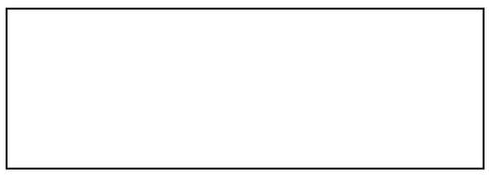
\includegraphics[height=2.5cm]{cake}
\end{center}

\end{problem}



\begin{problem}[Ordering fractions]
Use benchmarks and intuitive methods to arrange the fractions below in ascending order. Explain how you decided. (The point of this problem is to think more and compute less!):

\[
\frac 2 5 , \quad\quad \frac 1 3 , \quad\quad\frac 5 8 , \quad\quad \frac 1 4 , \quad \quad\frac 2 3 , \quad\quad  \frac 3 4, \quad\quad \frac 4 7.
\]

\end{problem}


\begin{problem}
Which of these fractions has the larger value?   {\bf Justify} your choice.  
\[
\frac{10001}{10002}   \text{  or }    \frac{10000001}{10000002}
\]

\end{problem}


\begin{problem}[Quick!]
Solve each division problem.  Look for a shortcut, and explain your work.

\[
\frac{251 + 251 + 251 +251}{4}
\]



\[
\frac{377 + 377 + 377 + 377 + 377}{5}
\]


\[
\frac{123123 + 123123 + 123123 + 123123 + 123123 + 123123}{3}
\]

\end{problem}



\begin{problem}[Cancellation]

Yoko says
\[
\frac{16}{64} = \frac 1 4
\]
because she cancels the sixes:
\[
\frac{1\cancel{6}}{\cancel{6}4} = \frac 1 4.
\]
But note:
\[
\frac{16}{64} = \frac{1 \cdot 16}{4\cdot 16} = \frac{1 \cdot \cancel{16}}{4\cdot \cancel{16}} = \frac 1 4.
\]
So is Yoko right?  Does her cancelation rule always work?
If it doesn't always work, can you find \emph{any other} example where it works?  Can you find \emph{every} example where it works?

\end{problem}

\begin{problem}
Jimmy says that a fraction doesn't change in value if you add the same amount to the numerator and the denominator.  Is he right?  If you were Jimmy's teacher, how would you respond?

\end{problem}


\begin{problem}
Shelly says that if $ab < cd$ then $\frac a b< \frac c d$.  Is Shelly's claim always true, sometimes true, or never true?  If you were Shelly's teacher, what would you say to her?

\end{problem}



 \begin{problem}
Jill, her brother, and another partner own a pizza restaurant.  If Jill owns $\frac 1 3$ of the restaurant and her brother owns $\frac 1 4$ of the restaurant, what fraction does the third partner own?
\end{problem}
 


\begin{problem}
John spent a quarter of his life as a boy growing up, one-sixth of his life in college, and one-half of his life as a teacher.  He spent his last six years in retirement.  How old was he when he died?
\end{problem}

\begin{problem}
Nana was planning to make a red, white, and blue quilt.
One-third was to be red and two-fifths was to be white. If
the area of the quilt was to be 30 square feet, how many
square feet would be blue?
\end{problem}
\fellow{add a picture of a Hawaiian quilt?}

\begin{problem}
 Rafael ate one-fourth of a pizza and Rocco ate one-third of it.  What fraction of the pizza did they eat?
\end{problem}


\begin{problem}[Tangrams]
Tangrams are  a seven-piece puzzle, and  the seven pieces can be assembled into a big square.

\begin{center}

\includegraphics[height=2.5cm]{tangramsquare}
\end{center}


\begin{enumerate} [(a)]
 \item
If the large square shown above is one whole, assign a fraction value to each of the seven tangram pieces.  Justify your answers. \\

 
\item
The tangram puzzle contains a small square.  If the small square (the single tangram piece)  is one whole, assign a fraction value to each of the seven tangram pieces.  Justify your answers. \\


 \item
The tangram set contains two large triangles.  If a large triangle (the single tangram piece)  is one whole, assign a fraction value to each of the seven tangram pieces.  Justify your answers. \\



 \item
The tangram set contains one medium triangle.  If the medium triangle (the single tangram piece)  is one whole, assign a fraction value to each of the seven tangram pieces.  Justify your answers. \\
 


 \item
The tangram set contains two small triangles.  If a small triangle (the single tangram piece)  is one whole, assign a fraction value to each of the seven tangram pieces.  Justify your answers. \\
 



 \end{enumerate}
 \end{problem}



\begin{problem}
Mikiko said her family made two square pizzas at home.  One of the pizzas was 8 inches on each side, and the other was 12 inches on each side.  Mikiko ate $\frac 1 4$ of the small pizza and $\frac 1{12}$ of the large pizza.  So she said  that she ate 
\[
\frac 1 4 + \frac 1 {12} 
\quad 
= 
\quad 
\frac 3{12} + \frac 1 {12} 
\quad 
= 
\quad 
\frac 4{12} 
\quad 
= 
\quad 
\frac 1 3
\]
of the pizza.
Do you agree with Mikiko's calculation?  Did she eat $\frac 1 3$ of her family's pizza?  Carefully justify your answer.
\end{problem}


\begin{problem}[Harmonic triangle]
Look at the triangle of numbers.  There are lots of patterns here!  Find as many as you can.  In particular, try to answer these questions:

\begin{enumerate}[(a)]
\item
What  pattern describes the first number in each row?
\item
How is each fraction related to the two fractions below it?
\item
Can you write down the next two rows of the triangle? 
\end{enumerate}

\begin{center}
\begin{tabular}{ccccccccc}
&&&& $\displaystyle\frac 1 1$ & & & &\\
&&&$\displaystyle\frac 1 2$&  &$\displaystyle\frac 1 2$ & & &\\
&&$\displaystyle\frac 1 3$&&$\displaystyle\frac 1 6$  & &$\displaystyle\frac 1 3$ & &\\
&$\displaystyle\frac 1 4$&&$\displaystyle\frac 1 {12}$ & & $\displaystyle\frac 1 {12}$& &$\displaystyle\frac 1 4$ &\\
$\displaystyle\frac 1 5$&&$\displaystyle\frac 1 {20}$&&$\displaystyle\frac 1 {30}$  & &$\displaystyle\frac 1 {20}$ & &$\displaystyle\frac 1 5$\\
\end{tabular}
\end{center}

\end{problem}



\begin{problem}[Let them eat cake!]
Marie made a sheet cake at home, but she saved some to bring to work and share with her co-workers the next day.  Answer these questions about Marie's cake.  (Draw a picture!)
\begin{enumerate}[(a)]
\item
Suppose Marie saved $\frac 1 2$ of the cake for her coworkers and the co-workers ate $\frac 3 4$  of this. What fraction of the entire cake did they eat?\\
\item
    What if Marie saved $\frac 1 6$ instead, and they ate $\frac 2 3$ of this?\\
    \item
    What if she saved $\frac 5 7$ of the cake and they ate $\frac 1 2$ of this?\\
    \end{enumerate}
 
\end{problem}





 \begin{problem}[Door prize]
An elementary school held a ``Family Math Night'' event, and 405 students showed up.  Two-thirds of the students who showed up won a door prize.  How many students won prizes?
\end{problem}


\begin{problem}[Working Backwards]
For each picture shown:
\begin{itemize}
\item
What multiplication problem is represented?
\item
What is the product?
\end{itemize}

\begin{center}

\includegraphics[height=3.5 cm]{FracMult2}
\qquad\qquad\qquad
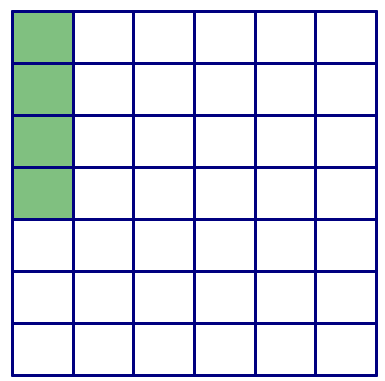
\includegraphics[height=3.5 cm]{FracMult3}
\end{center}
\end{problem}





 \begin{problem}[Depreciation]
A piece of office equipment was purchased for \$60,000.  Each year, it depreciates in value.  At the end of each year, the equipment is worth $ \frac{9} {10} $ what it was worth at the start of the year.
How much is the equipment worth after 1 year?  After 2 years?  After 5 years?
\end{problem}

 
\begin{problem}[How close can you get?]
Using only the digits 0, 1, 2,\dots , 9 at most once each in place of the variables, find the value closest to 1.  For each problem, justify your solution.  How do you \emph{know} it's closest to 1?
\begin{enumerate}[(a)]
\item
$\displaystyle \frac a b$\\

\item
$\displaystyle \frac a b \cdot \frac c d$\\

\item
$\displaystyle \frac a b \cdot \frac c d \cdot \frac e f$\\

\end{enumerate}

\end{problem}





 \begin{problem}[Community garden]
A town plans to build a community garden that will cover $\frac 2 3$ of a square mile. They would like to situate it on a pasture of an old  farm. One dimension of the garden area will be determined by a fence that is $\frac 3 4$ of a mile long. If the garden is a rectangle, how long is the other side?


\end{problem}






 \begin{problem}[Planting wheat]
Nate used $90 \frac 1 2$ pounds of seed to plant $1 \frac 1 4$ acres of land in spring wheat.  How many pounds of seed is he using per acre?
\end{problem}

 

\begin{problem}
The family-sized box of laundry detergent contains 35 cups of detergent.  Your family's  machine requires  $1 \frac 1 4$ cup per load.  How many loads of laundry can your family do with one box of detergent?
\end{problem}



\begin{problem}
At the start of each semester, $\frac 5 6$ of all Math 111 students work out at least three times each week.    By the middle of the semester, $\frac 4 5 $ of those students are still working out regularly.  By the time finals rolls around, $\frac 9{10}$ of those students still hit the gym three times each week.  If 36  students are working out regularly during finals, how many were enrolled in Math 111 at the start of the semester?
\end{problem}


\begin{problem}
Jessica bikes to campus every day.  When she is one-third of the way between her home and where she parks her bike, she passes a grocery store.   When she is halfway to school, she passes a Subway sandwich shop.  This morning, Jessica passed the grocery store at 8:30am, and she passed Subway at 8:35am.  What time did she get to campus?
\end{problem}

\begin{problem}
If you place a full container of flour on a balance scale and place on the other side a $\frac 1 3$ pound weight plus a container of flour (the same size) that is $\frac 3 4 $ full, then the scale balances.  How much does the full container of flour weight?

\fellow{add a picture?  also if it makes sense for any of the other problems...}
\end{problem}


\begin{problem}
Geoff spent $\frac 1 4$ of his allowance on a movie.  He spent $\frac{11}{18}$ of what was left on snacks at school.  He also spent \$3 on a magazine, and that left him with $\frac 1{24}$ of his total allowance, which he put into his savings account.  How much money did Geoff save that week?
\end{problem}


\begin{problem}
Lily was flying to San Francisco from Honolulu.  Halfway there, she fell asleep.  When she woke up, the distance remaining was half the distance traveled while she slept.  For what fraction of the trip was Lily asleep?
\end{problem}







\section{Egyptian Fractions}

Scholars of ancient Egypt (about 3000 B.C.) were very practical in their approaches to
mathematics and always sought answers to problems that would be of most
convenience to the people involved. This led them to a curious approach to thinking
about fractions.

\begin{example}[Egyptian fractions for $\frac 7{12}$]
Consider the problem: Share 7 pies among 12 boys.
Of course, given our model for fractions, each boy is to receive the quantity ``$\frac 7 {12}$''
But  this answer has little intuitive feel.

Suppose we took this task as a very practical problem. Here are the seven pies:
\begin{center}
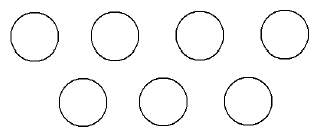
\includegraphics[height=3cm]{sevenpies}
\end{center}

Is it possible to give each of the boys a whole pie? No. 

How about the next best
thing --- can  each boy get half a pie? Yes! There are certainly 12 half pies to dole out. There
is also one pie left over yet to be shared among the 12 boys. Divide this into
twelfths and hand each boy an extra piece.

\begin{center}
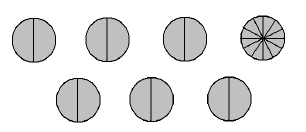
\includegraphics[height=3cm]{sevenpies_split}
\end{center}

So each boy gets $\frac 1 2 + \frac 1{12}$ of a pie, and it is indeed true that
\[
\frac{7}{12} = \frac 1 2 + \frac 1 {12}.
\]
(Check that calculation\dots don't just believe it!)

\end{example}

\begin{thinkpair*}\ 
\begin{enumerate}
\item
How do you think the Egyptians might have shared five pies among six boys?
\begin{center}
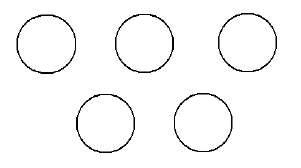
\includegraphics[height=3cm]{fivepies}
\end{center}

\item
How would they have shared seven pies among 12 boys?

\end{enumerate}

\end{thinkpair*}

The Egyptians (probably) weren't particularly concerned with splitting up pies.  But in fact, they did have a very strange (to us) way of expressing fractions. We know this by examining the  Rhind Papyrus.  This ancient document indicates that fractions were in use as many as four thousand years ago in Egypt, but the Egyptians seem to have worked primarily with \emph{unit fractions}.  They insisted on writing all of their fractions as sums of fractions with
numerators equal to 1, and they insisted that  the denominators of the fractions were all different.

\fellow{Can you add a (SHORT) blurb about the Rhind Papyrus and a picture?  Like the Polya blurb that Ryan added to the Problem Solving chapter.}

\begin{example}[Egyptian fractions]
The Egyptians would not write $\frac 3{10}$, and they would not even write $\frac 1{10} + \frac 1{10} + \frac 1{10}$.  Instead, they wrote 
\[
\frac 1 4 + \frac 1{20}.
\]


The Egyptians would not write $\frac 5{7}$, and they would not even write $\frac 1{7} + \frac 1{7} + \frac 1{7} + \frac 1{7} + \frac 1{7}$.  Instead, they wrote 
\[
\frac 1 2 + \frac 1 5 + \frac 1{70}.
\]

(You should check that the sums above give the correct resulting fractions!)
\end{example}



\begin{problem}[$\frac 2 n$]
Write the following as a sum of two \emph{different} unit fractions.  Be sure to check your answers.
\[
\frac 2 3,
\qquad\qquad\qquad
\frac 2 9,
\qquad\qquad\qquad
\frac 2 {15},
\qquad\qquad\qquad
\frac 2{25}.
\]
Can you express this process as a general algorithm?


\end{problem}


\begin{problem}[Fractions bigger than $\frac 1 2$]
Write the following as a sum of distinct unit fractions.  (``Distinct'' means the fractions must have different  denominators.)  Note that you may need to use more than two unit fractions in some of the sums.  Be sure to check your answers.
\[
\frac 3 4,
\qquad\qquad\qquad
\frac 5 6,
\qquad\qquad\qquad
\frac 3 5,
\qquad\qquad\qquad
\frac 5 9.
\]
Can you express this process as a general algorithm?


\end{problem}






\begin{problem}[Challenges]
Write the following fractions as Egyptian fractions.  
\[
\frac{17}{20},
\qquad\qquad\qquad
\frac 3 7.
\]
Can you find a general algorithm that will turn \emph{any fraction at all} into an Egyptian fraction?


\end{problem}






\section{Algebra Connections}
In an advanced algebra course students are often asked to work with complicated
expressions like:
\[
\frac{\frac 1 x + 1}{\frac 3 x}.
\]
We can make it look friendlier by following exactly the same technique of the
previous section. In this example, let's multiply the numerator and denominator each
by $x$. (Do you see why this is a good choice?) We obtain:
\[
\frac{\left(\frac 1 x + 1\right)\cdot x}{\left(\frac 3 x\right)\cdot x}
\quad
=
\quad
\frac{1+x}{3},
\]
and $\frac{1+x}{3}$ is much less scary.

\begin{example}
As another example, given:
\[
\frac{\frac 1 a - \frac 1 b}{ab},
\]
one might find it helpful to multiply the numerator and the denominator each
by $a$ and then each by $b$:
\[
\frac{\left(\frac 1 a - \frac 1 b\right)\cdot a \cdot b}{\left(ab\right)\cdot a \cdot b}
\quad
=
\quad
\frac{b-a}{a^2b^2}.
\]

\end{example}


\begin{example}
For 
\[
\frac{\frac 1 {(w+1)^2} - 2}{\frac 1 {(w+1)^2} +5},
\]
it might be good to multiply top and bottom each by $(w+1)^2$.  (Why?)
\[
\frac{\left(\frac 1 {(w+1)^2} - 2\right)\cdot (w+1)^2}{\left(\frac 1 {(w+1)^2} +5\right)\cdot (w+1)^2}
\quad
=
\quad
\frac{1 - 2(w+1)^2}{1+5(w+1)^2}.
\]


\end{example}

\subsection*{On Your Own}
Can you make each of these expressions look less scary?

\[
\frac{2-\frac 1 x}{1 + \frac 1 x},
\qquad\qquad
\frac{\frac1{x+h} + 3}{\frac 1{x+h}},
\qquad\qquad
\frac{1}{\frac 1 a + \frac 1 b},
\qquad\qquad
\frac{\frac{1}{x+a} - \frac 1 x} a.
\]






\section{What is a Fraction? Part 3}
So far, we have no single model that makes sense of fractions in all contexts.  Sometimes a fraction is an action (``Cut this in half.'')  Sometimes it is a quantity (``We each get $2/3$ of a pie!'')  And sometimes we want to treat fractions like \emph{numbers}, like ticks on the number line in-between whole numbers.

We could say that a fraction is just a pair of numbers $a$ and $b$, where we require that $b \neq 0$.  We just happen to write the pair as $\frac a b$.  

But again this is not quite right, since whole infinite collection of pairs of numbers represent
the same fraction!  For example:
\[
\frac 2 3 = \frac 4 6 = \frac 6 9 = \frac 8 {12} = \cdots
\]
 So a single fraction is actually a
whole infinite class of pairs of numbers that we consider ``equivalent.''
 


How do mathematicians think about fractions?  Well, in exactly this way.  They think of pairs of numbers written as $\frac a b$, where we remember two important facts:
\begin{itemize}
\item
$b \neq 0$, and
\item
$\frac a b$ is really shorthand for a whole infinite class of pairs that look like $\frac{xa}{xb}$.

\end{itemize}
This is a hefty shift of thinking: The notion of a ``number'' has changed from being a
specific combination of symbols to a whole class of combinations of
symbols that are deemed equivalent.


Mathematicians then \emph{define} the addition of fractions to be given by the daunting rule:
\[
\frac a b + \frac c d = 
\frac{ad +bc}{bd}.
\]
This obviously motivated by something like the ``Pies Per Boy Model.''   But if we just \emph{define} things this way, we must worry
about \emph{proving} that choosing different representations for $\frac a b$ and $\frac c d$
lead to the same
final answer. 

For example, it is not immediately obvious that
\[
\frac 2 3 + \frac 4 5
\qquad
\text{and}
\qquad 
\frac 4 6 + \frac{40}{50}
\]
give
answers that are equivalent.  (Check that they do!)

They also \emph{define} the product of fractions as:
\[
\frac a b \cdot \frac cd = \frac{ac}{bd}.
\]
Again, if we start from here, we have to \emph{prove} that all is
consistent with different choices of representations.

Then mathematicians establish that the axioms of an arithmetic system hold with these
definitions and carry on from there!  (That is, they check that addition and multiplication are both commutative and associative, that the distributive law holds, that all representations of 0 act like an additive identity, and so on\dots)

This is abstract, dry and not at all the best first encounter to offer students on the topic of
fractions. And, moreover, this approach completely avoids the question as to what a
fraction really means in the ``real world.'' But it is the best one can do if one is to be
completely honest. 

The definitions are certainly motivated by the type of work we did in this chapter, but in the end one can't explain why these rules are the way they are.

\begin{thinkpair*}
So\dots what is a fraction, really?  How do you think about them?  And what is the best way to talk about them with elementary school students?
\end{thinkpair*}



  
